%! Author = helgaingim
%! Date = 8.8.2023
\documentclass[
    NAME={Dr. Helga Ingimundardóttir},
    EMAIL={helgaingim@hi.is},
    FACULTY={Industrial Engineering},
    TITLE={Pushing Boundaries: A Data-Driven Dive into `Legend of the Ice People'},
    SUBTITLE={Unravel the unexpected synergy of literature and data science},
    SEMINAR={Haustráðstefna Advania},
    DATE={September 8, 2023}
    ]{hi-latex/hi-beamer}
%\setbeameroption{show notes}

\usepackage{media9}
\usepackage[scale=2]{ccicons}

\newcommand{\customframe}[3][]{
    \usebackgroundtemplate{
        \tikz[overlay,remember picture]
        \node[opacity=0.3, at=(current page.center)] {
            \includegraphics[width=\paperwidth,height=\paperheight]{#2}
        };
    }
    \ifx&#1&
        \section{#3}
    \fi
    \addtobeamertemplate{frametitle}{\vskip3cm}{} % Adjust the frametitle position for this slide only
    \begin{frame}[plain]{#3}
        #1
    \end{frame}
    \addtobeamertemplate{frametitle}{\vskip-3cm}{} % Reset the frametitle template to default
    \usebackgroundtemplate{}  % Reset the background for the following frames
}

\begin{document}

%\toggleColor
% Outline
\customframe[\tableofcontents]{../rek-data-beers/figures/dalle-book-2}{Outline}

% Introduction
\customframe{../rek-data-beers/figures/dalle-book-3}{Introduction}
\begin{frame}{About Me}
\note{
    I hold a Ph.D. in Computational Engineering, a field that bridges computation and practical applications.

    \scriptsize{
      Over the years, I've played various roles. Let's take a walk down memory lane:
      My journey began as a Software Developer at Valka, which later evolved into Marel. I contributed to their revolutionary waterjet cutter's software.
      Venturing into databases, I became an SQL Consultant at AGR.
      After defending my PhD, my next destination was deCODE genetics, diving into genetic research and long-range sequencing.
      The gaming world beckoned after COVID, and I joined CCP Games as a Data Scientist.
      Travelshift saw me as their Head of AI Research, where I tackled challenges similar to those during my PhD days.
      \textbf{Presently}, I have the privilege of mentoring young minds as an Assistant Professor in the Industrial Engineering Department at the University of Iceland.
    }

    \begin{itemize}
        \item A notable highlight of my career was my talk on the \emph{Legend of the Ice People} at Reykjavík Databeers. This talk drew inspiration from a literary podcast I hosted, \emph{ÍSKISUR}. A modern take on literary analysis, it was a thrilling experience.
        \item On being invited to this distinguished conference to discuss ÍSFÓLKIÐ, many might deem it 'trivial'. Yet, as we're about to delve into, ÍSFÓLKIÐ is far from mundane as the data will show.
    \end{itemize}
}

I am a \emph{Ph.D.} in Computational Engineering.
\vspace{1em}
\begin{columns}[T] % alignment of columns
  \begin{column}{0.6\textwidth} % adjust width to your liking
    Past Roles:
    \begin{itemize}
      \item Software Developer at Valka
      \item SQL Consultant at AGR
      \item Research Scientist at deCODE genetics
      \item Data Scientist at CCP Games
      \item Head of AI Research at Travelshift
    \end{itemize}
  \end{column}

  \begin{column}{0.35\textwidth} % adjust width to your liking
      \begin{exampleblock}{Current Role:}
        \emph{Assistant Professor} in the Industrial Engineering Department at the University of Iceland
      \end{exampleblock}
  \end{column}
\end{columns}

  \vfill
  \begin{block}{Signature Talk}
      Analysis of \emph{Legend of the Ice People} a.k.a. \emph{ÍSFÓLKIÐ} for Reykjavík Databeers \#6.

      \vspace{0.5em}

      Inspired by the literary podcast I co-hosted, \emph{ÍSKISUR}.
  \end{block}
\end{frame}


\begin{frame}{A Surprising Insight}
\note{
  \begin{itemize}
    \item When I presented at Databeers last June, I planned for a 7-min lightning talk.
    \item However, the audience's reaction took me by surprise.
    \item They were intrigued by the data-driven angle I took on ÍSFÓLKIÐ.
    \item Many expressed astonishment at the idea of applying data-driven approaches to literature.
    \item The discussions were so engaging that, with permission, we went well over time, turning that brief talk into a 45-minute in-depth discussion.
    \item So if there's one key \textbf{takeaway} from my experience, it's this:
    Data is all around us. With the right perspective, we can find and interpret data in the most unexpected domains.
    \item Be open to data, and it can unlock fresh insights and lively discussions, as I found out!
  \end{itemize}
}

\begin{columns}[T]

  \begin{column}{0.6\textwidth}
    What surprised most about my presentation at \emph{Reykjavík Databeers} was the audience's reaction:
    \begin{itemize}[<+->] % <+-> will animate the items to appear one-by-one
      \item They didn't expect a data-driven angle to \emph{ÍSFÓLKIÐ}.
      \item Astonished by \emph{several} data-driven approaches to literature.
      \item Analytical framework shed new light and perspectives.
    \end{itemize}
  \end{column}

  \begin{column}{0.4\textwidth}
    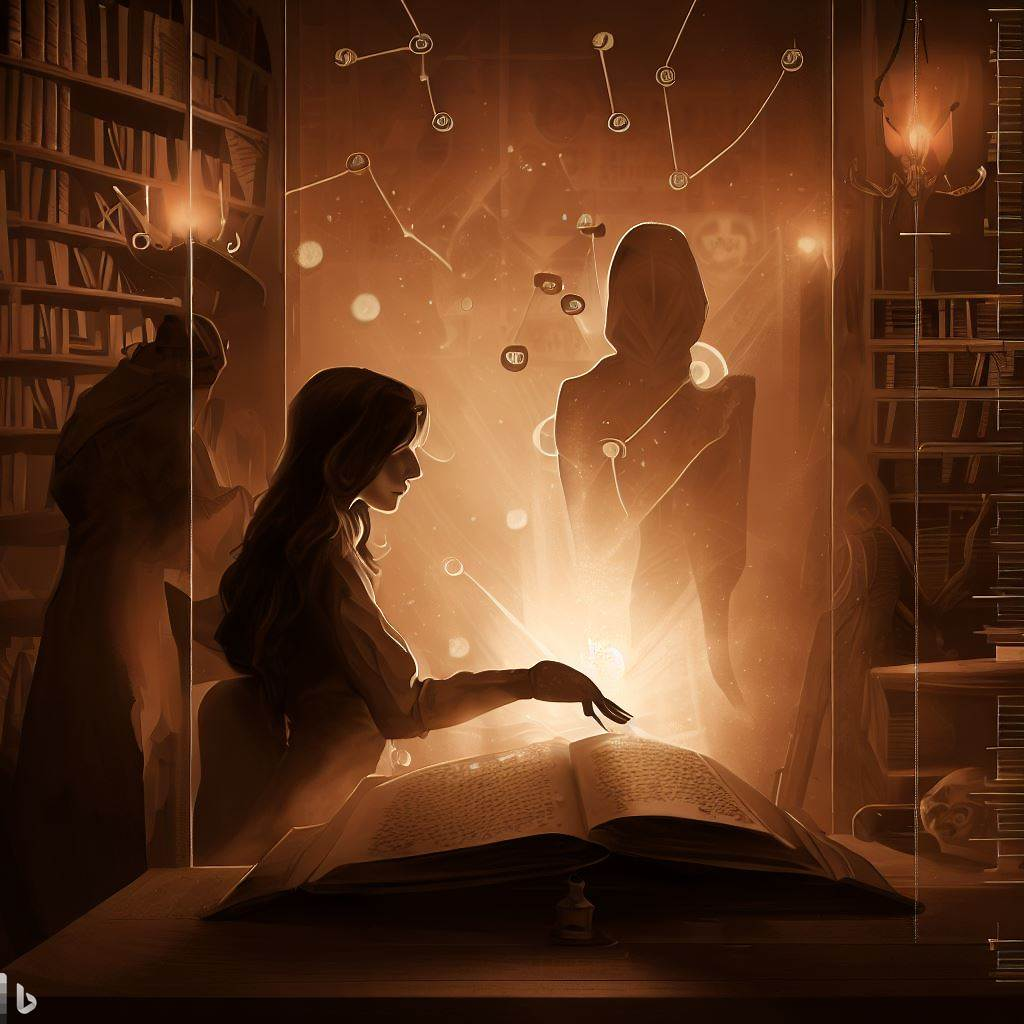
\includegraphics[width=\textwidth]{../figures/dalle-insights} % Consider an image that represents surprise or insight.
  \end{column}

\end{columns}

\vspace{0.5em}

\begin{block}{Take-Home Message}
Anything can be data-driven with the right mindset. Data is everywhere; it's about looking for it and using it. Embrace data for fresh insights, even in unexpected domains.
\end{block}

\end{frame}


\begin{frame}{Backstory: From Cat Memes to Podcasts} \note{
In 2012, I stumbled upon the world of \textbf{internet cats} and was immediately \textit{captivated}.
It began innocently enough: I'd seek out \textbf{quirky cat memes} to share on my social platforms.
But soon, it became more than just a hobby. My friends began \textit{discreetly} forwarding me cat images,
and I'd then share them with the world. Without even realizing it, I became a well known \underline{internet cat lady}.

\bigskip  % A pause here for a slight change in topic

By 2016, I discovered a podcast named \textbf{My Dad Wrote A Porno}. It was both \textit{hilarious} and spellbinding.
Inspired by their creativity, my friends and I wanted to start our own show.
But we faced a problem: none of our parents wrote erotic fiction. So, we \textbf{improvised} and decided to read \emph{ÍSFÓLKIÐ},
putting our own twist on it.

\bigskip  % Another pause for a change in topic

To incorporate my love for cats, I introduced a special segment at the end of each episode titled
\emph{Internet Cat of the Week}. And that's how two of my passions \underline{converged}.
    }
    \begin{itemize}
        \item 2012: Became the internet cat lady -- Memes $\Rightarrow$ Friends' Cat pics.
        \item 2016: Inspired by \emph{My Dad Wrote A Porno} podcast.
        \item Solution: Read \emph{ÍSFÓLKIÐ} with our twist.
        \item Special Segment: \emph{(Internet) Cat of the Week}.
    \end{itemize}
    \vfill


\begin{columns}
    \begin{column}{0.8\textwidth}
        \begin{exampleblock}{TL;DL: My Dad Wrote a Porno (2015--)}
            A 3-time Webby Award-winning comedic podcast where host Jamie Morton reads his father's amateur erotic novel. With friends James Cooper and Alice Levine, they hilariously dissect awkward, improbable tales blending family and risqué fiction.
        \end{exampleblock}
    \end{column}
    \begin{column}{0.2\textwidth}
        
\includegraphics[width=\textwidth]{../figures/my-dad-wrote-a-porno}
    \end{column}
\end{columns}


\end{frame}

\begin{frame}{About ÍSKISUR}
    \note{
      \textbf{Introduction to ÍSKISUR:}
      ÍSKISUR is a rather unique podcast, combining two things many wouldn't expect to find together: literature and, believe it or not, cats. Each episode we dive into the world of \emph{The Legend of the Ice People} by Margit Sandemo. This series is filled with both erotic and surreal elements, making it a treasure trove for lively discussions.

      \textbf{Episode Structure:}
      But our podcast doesn't end with just discussing the book. As a nod to my personal fondness for cats, every episode concludes with a delightful segment on internet cats.

      \textbf{Graphics and Podcast Members:}
        Now, if you look to your left, you'll see an iconic image from the Internet Cat Festival held back in 2013. This memorable meeting between Grumpy Cat and Lil Bub truly epitomizes the fun spirit of our show.
        And to your right is our official podcast image on Storytel. It features myself alongside my amazing co-hosts Birna and Kristín.
        \textbf{Disclaimer}: despite our deep dives into the book series, none of us claim to be actual cats or literary experts.
    }
    \begin{columns}[T]
        \begin{column}{0.55\textwidth}
            \begin{itemize}
                \item A literary and feline entertainment podcast*
                \item Discuss the erotic and surreal book series \emph{The Legend of the Ice People} by Margit Sandemo
                \item Each episode covers part of a book from the series and concludes with a segment on internet cats
            \end{itemize}
            \vspace{12pt}

            \centering
            
\includegraphics[width=.7\textwidth]{../rek-data-beers/figures/internet-cats}
            \tiny{via @iamlilbub}

            \scriptsize{Grumpy Cat first meeting Lil Bub\\Internet Cat Festival, 2013}
        \end{column}x
        \begin{column}{0.45\textwidth}
            \centering
            
\includegraphics[width=\textwidth]{../rek-data-beers/figures/podcast_image.jpg}
            \vfill
            Birna, Kristín, and dr.~Helga\\
            \vspace{12pt}
            \footnotesize{*\textit{None of the hosts are actually cats or literary experts.}}
        \end{column}
    \end{columns}
\end{frame}

\begin{frame}{About ÍSFÓLKIÐ}
    \note{
    \begin{itemize}
        \item ÍSFÓLKIÐ: A 47-volume family saga in historic Scandinavia, filled with mystical elements.
        \item Central is Silja and her family, marked by an age-old curse from Þengill.
        \item While Silja's bond with Þengill the Good deepens the curse's influence, their descendants wrestle with its implications.
        \item The family's enduring struggle is with Þengill the Bad, culminating in an epic confrontation.
        \item Throughout, spirits and mystical mandrake root play crucial roles, assisting the family.
    \end{itemize}
    }

    \begin{columns}[T]
        \begin{column}{0.65\textwidth}
            \begin{itemize}
                \item Epic 47-volume tale set in historic Scandinavia with fantasy elements.
                \item The tale revolves around a \emph{curse} originating from malevolent Þengill.
                \item Silja, an ordinary woman, becomes intertwined with the curse through Þengill the Good.
                \item Their offspring, destined to face Þengill the Bad's rising evil, represent each book's focus.
                \item Culmination: The family's ultimate confrontation with Þengill the Bad.
                \item Spirits and mandrake root: Mysterious aids interwoven into the narrative.
            \end{itemize}
        \end{column}

        \begin{column}{0.35\textwidth}
            
\includegraphics[width=\textwidth]{../figures/dalle-ísfólkið}
            {\scriptsize\begin{itemize}
                \item \emph{Silja}: Innocent matriarch of the cursed family.
                \item \emph{Þengill the Good}: Bearer of the curse, forsakes celibacy for Silja.
                \item \emph{Þengill the Bad}: Ever-strengthening evil antagonist.
            \end{itemize}}
        \end{column}
    \end{columns}
\end{frame}

\begin{frame}{Exploring Different Formats}
\note{
\scriptsize{
    \textbf{The Written format:}
    \begin{itemize}
        \item The series became a cultural touchstone in the 80s, captivating a generation. Its influence was so profound that it led readers to name their children after the characters.
        \item Its relevance persisted, prompting a re-translation in 2007 for newer readers.
    \end{itemize}
    \textbf{The Audio format:}
    \begin{itemize}
        \item The audiobooks, introduced in 2017, quickly became titans on Storytel, showcasing the series' undying charm.
        \item Their widespread success transformed them into one of the most sought-after listens on the platform.
        \item ÍSKISUR, initially a simple bookclub discussion among friends on Alvarpið, the podcast breathed a fresh, candid perspective into the series.
        \item Recognizing the value and its potential, Storytel approached us. Moved by the soaring popularity of the audiobooks, they offered professional editing, and a soundstage for recording, elevating our small DIY project to professional production standards.
    \end{itemize}
}
}


  \begin{columns}[T] % alignment of columns
    \begin{column}{0.32\textwidth}
        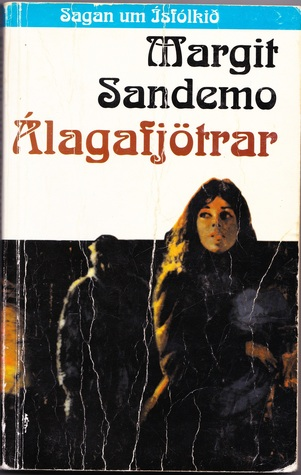
\includegraphics[width=.48\textwidth]{../figures/álagafjötrar_margit}
        
\includegraphics[width=.48\textwidth]{../figures/álagafjötrar_jentas}\\
      \textbf{The Written Books}
      \begin{itemize}
          \item 80s cult phenomenon.
          \item Re-translated in 2007.
          \item Influenced children's names.
      \end{itemize}
    \end{column}
\pause
    \begin{column}{0.32\textwidth}
        
\includegraphics[width=\textwidth]{../figures/álagafjötrar_storytel}\\
      \textbf{The Audio Books}
      \begin{itemize}
        \item Top content on \emph{Storytel}.
        \item Widely listened to.
      \end{itemize}
    \end{column}
\pause
\begin{column}{0.32\textwidth}
  
\includegraphics[width=\textwidth]{../figures/álagafjötrar_ískisur}\\
      \textbf{The Podcast}
      \begin{itemize}
        \item Small friend-led bookclub.
        \item Started on \emph{Alvarp Nútímans}.
        \item Moved to \emph{Storytel}.
      \end{itemize}
    \end{column}
  \end{columns}
\end{frame}


\begin{frame}{Timeline for the Legend of the Ice Cat-People}
\note{
\tiny{
    \textbf{Visual Overview:}
    The slide visually encapsulates the publication journey of both the written form and its newer audio adaptations.
    There are several life events annotated on the timeline which I'll further discuss and expand upon in subsequent sections.

    \textbf{Upper half: Book Series}
    \begin{itemize}
        \item Showcases the staggered release of the entire 47-part saga in Iceland.
    \end{itemize}

    \textbf{Lower half: Audio Adaptations}
    \begin{itemize}
        \item The journey began in earnest in fall 2016, when initial podcast episodes were recorded, but remained unreleased as we refined our production skills.
        \item ÍSKISUR made its debut on Alvarpið's 3rd anniversary in 2017, our podcast was featured alongside renowned titles such as Hefnendur and Englaryk.
        \item It's noted, this is before the major e-book release on Storytel. I like to think of ourselves as trendsetters.
        \item Although a hiatus intervened due to scheduling clashes and health issues, our passion project took a fortunate turn in 2019. Storytel recognized the podcast's potential and extended a collaboration offer. This meant not only compensation for our efforts but also relief from cumbersome post-production tasks, as we were living in different part of the country, and later different countries.
        \item With Storytel continuing the distribution of the audiobooks into fall of 2019.
        \item Our ÍSKISUR series reached its conclusion at the end of 2020. This marked the end of our intense four-year dive into Margit's world.
    \end{itemize}

}}
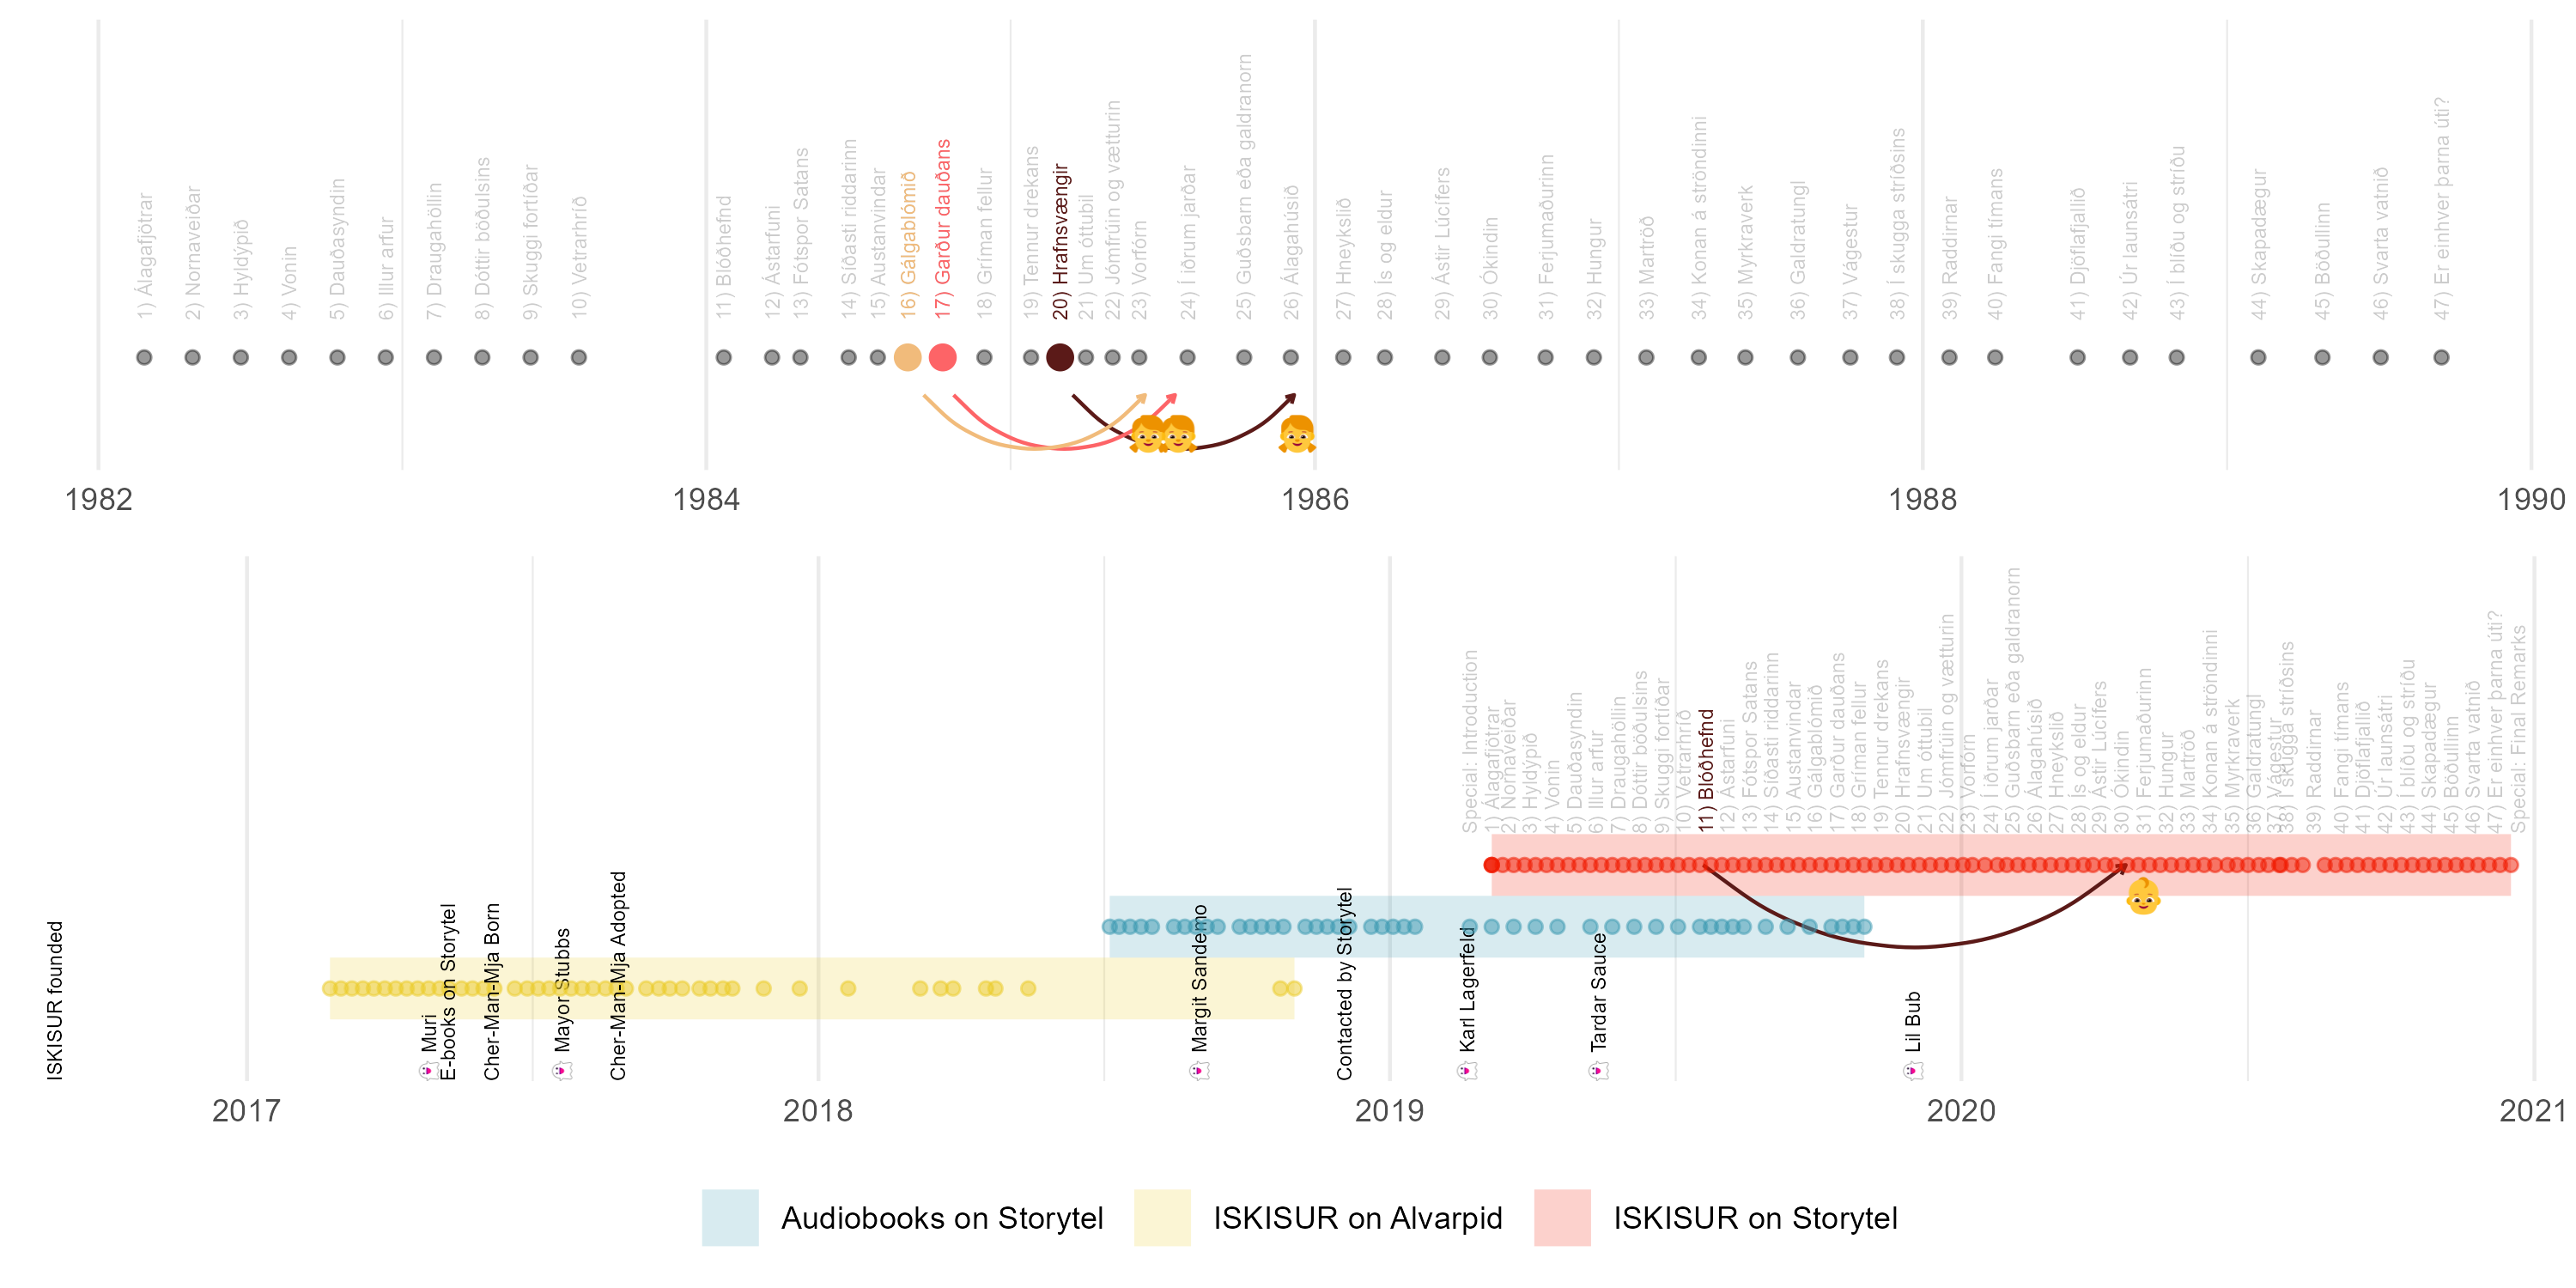
\includegraphics[width=\textwidth]{../rek-data-beers/R/figures/timeline}
\end{frame}


\customframe{../rek-data-beers/figures/dalle-book-4}{Written Books}
\begin{frame}{Margit Sandemo, 1924--2018}
    \note{\tiny{
    The person behind the book series is the renowned novelist \emph{Margit Sandemo}.
    Here's Margit at the book signing event for the re-translation of \emph{Álagafjötrar} held at Eymundsson in 2007.
    A book that began the epic journey of the cursed family we're exploring today.

    \begin{itemize}
    \item Margit Sandemo was born in 1924 and lived a remarkable life until her passing in 2018 at the age of 94—her journey intersected with our ÍSKISUR project.
    \item As a Norwegian-Swedish author, her literary impact in the Nordic countries is undeniable and enduring.
    \item Her father, a Norwegian poet, bequeathed her a literary lineage. Furthermore, she intriguingly claimed lineage to a Nobel Prize-winning author through an alleged affair.
    \item Although surrounded by literature, Margit embarked on her authorial journey at 40, a testament to the adage, 'it's never too late.'
    \item From the 1980s onwards, her novels consistently graced the best-seller lists in the Nordics, showcasing her unparalleled storytelling.
    \item Among her notable works, three series stand prominent:
        \emph{The Legend of the Ice People} from the 1980s, which is our primary topic for today.
        \emph{The Warlock} in the early 1990s, delving into mystical elements, particularly one witch lineage.
        \emph{The Legend of the Realm of Light} in the late 1990s, following the later generations of the Ice People and their continued struggles against dark forces.
    \item Margit seamlessly integrated history and fiction. Drawing inspiration from her noble Oxenstierna ancestors,
    she weaved them into pivotal historical events like the Thirty Years' War.
    Moreover, her fictional world was populated with mythological elements, with Lucifer finding a home in Dimmuborgir,
    which served not just as a backdrop but also as an inadvertent advertisement for Iceland abroad.
    \emph{Such fusion of history, legacy, and mythology provided her readers with a rich, resonating narrative}.
    \item The Ice People remained her muse for nearly two decades, a testament to her commitment and creativity.
\end{itemize}

}}

    \begin{columns}[T]
        \begin{column}{0.6\textwidth}
            \begin{itemize}
                \item Norwegian-Swedish author
                \item Father was a Norwegian poet, Anders Underdal
                \item Claimed lineage to Nobel Prize-winning author Bjørnstjerne Bjørnson
                \item First published at forty years old
                \item Best-selling author in the Nordic countries since the 1980s
            \end{itemize}
            \vfill
            \begin{scriptsize}
                \begin{table}
                    \begin{tabular}{rcc}
                        \textbf{Notable Book Series}     & \textbf{Years} & $n$ \\ \midrule
                        The Legend of the Ice People     & 1982--89       & 47  \\
                        The Warlock                      & 1991--94       & 15  \\
                        The Legend of the Realm of Light & 1995--99       & 12
                    \end{tabular}
                \end{table}
            \end{scriptsize}
        \end{column}
        \begin{column}{0.4\textwidth}
            \centering
            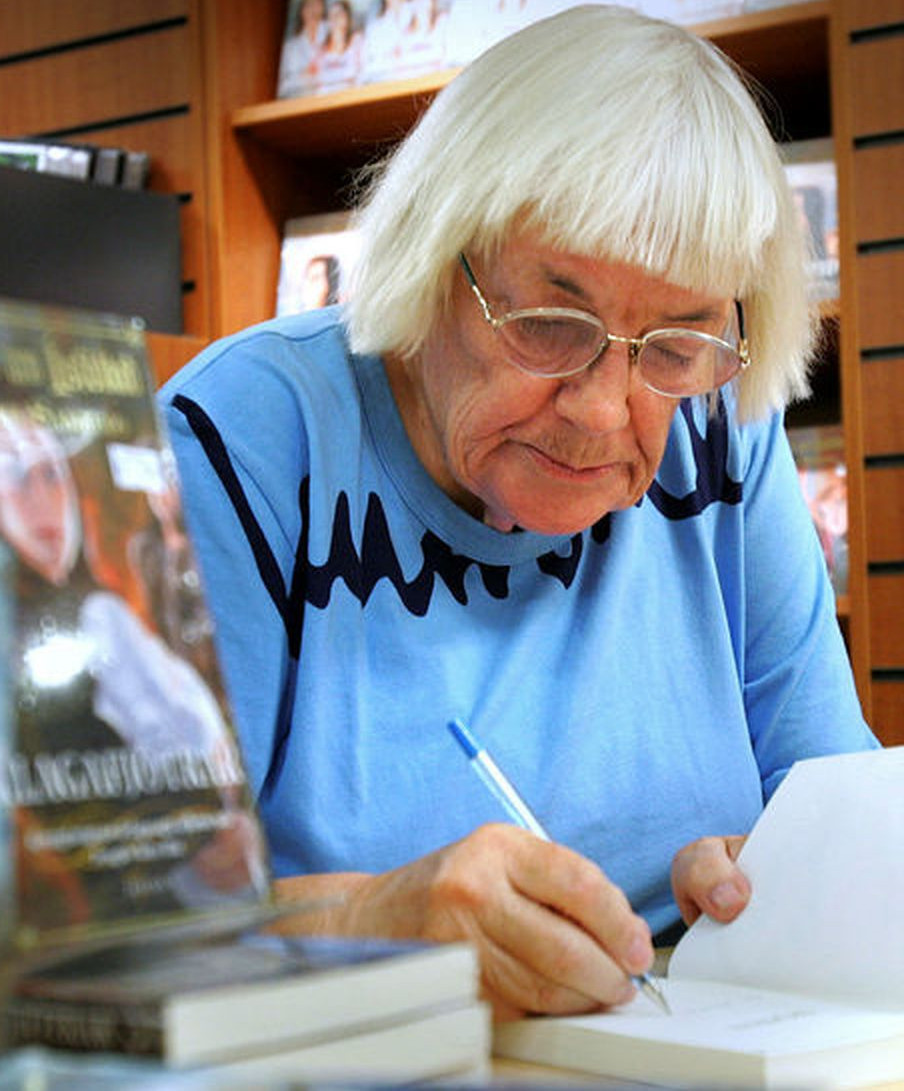
\includegraphics[width=\textwidth]{../rek-data-beers/figures/margit_sandemo}
            \begin{tiny}
                mbl.is/Þorvaldur Örn Kristmundsson
            \end{tiny}

            \vfill
            Margit signing \emph{Álagafjötrar} in Eymundsson, 2007
        \end{column}
    \end{columns}
\end{frame}

\begin{frame}{Publications}

    \note{
        The scatter plot illustrates the timeline of Margit's book publications in Iceland over an intense 8-year span.

        Throughout this period, Margit's prolificacy is evident: a remarkable 47 books were published,
        averaging a release every 8-9 weeks, with Tuesdays often being the chosen release day.

        Some discernible patterns from the data:
        \begin{itemize}
            \item Margit had a penchant for consistency, often sticking to a structure of 14 chapters (with few exceptions) for each book.
            \item As the series advanced, a decrease in the length of the books is observed.
            This aligns with her reflections in the final epilogue, \emph{Is There Anybody Out There?} (an homage to Pink Floyd's \emph{The Wall}).
            \item There she discloses her struggle with maintaining the narrative's momentum, hinting at writer's fatigue and the challenge of keeping the saga engaging.
        \end{itemize}
}
    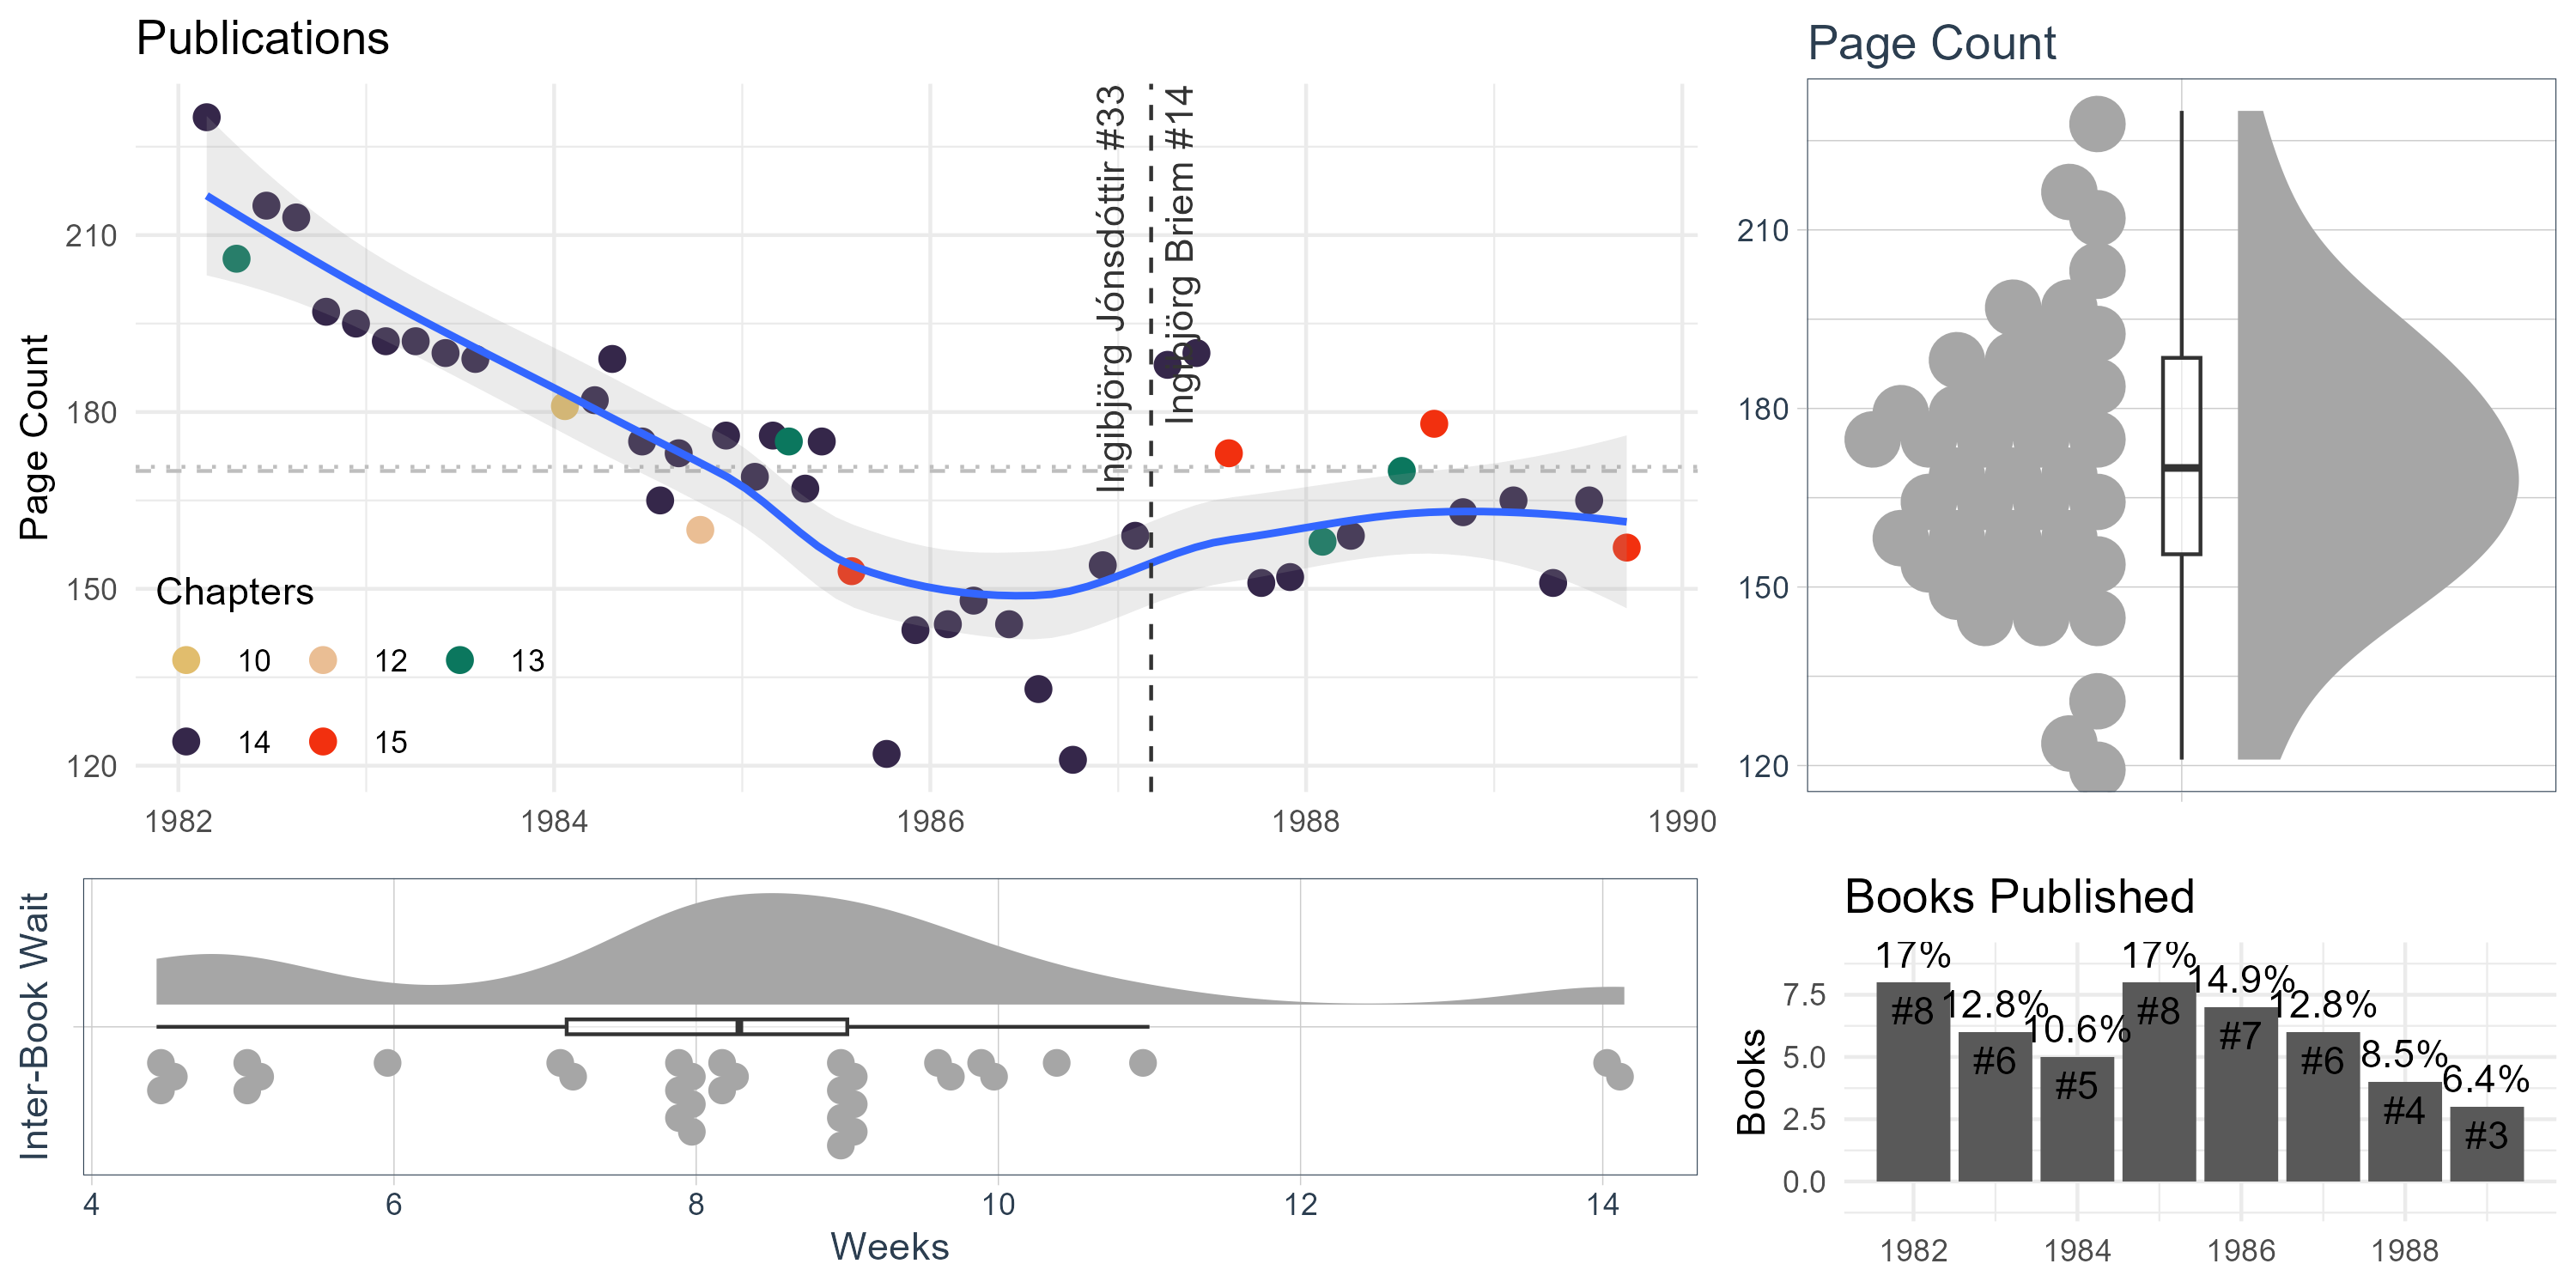
\includegraphics[width=\textwidth]{../rek-data-beers/R/figures/margit_count}
    \vspace{-24pt}
    \begin{itemize}
        \item 47 books, 652 chapters, 8,023 pages, 8 years
        \item Average book length: 170 pages (avg. 13.9 chapters)
        \item Released 1 book every 2 months (avg. 57.9 days), usually on Tue.
    \end{itemize}
\end{frame}


\customframe{../rek-data-beers/figures/dalle-book-5}{Audio Books}
\begin{frame}
    \frametitle{Audiobooks on Storytel: Active Fanbase}
    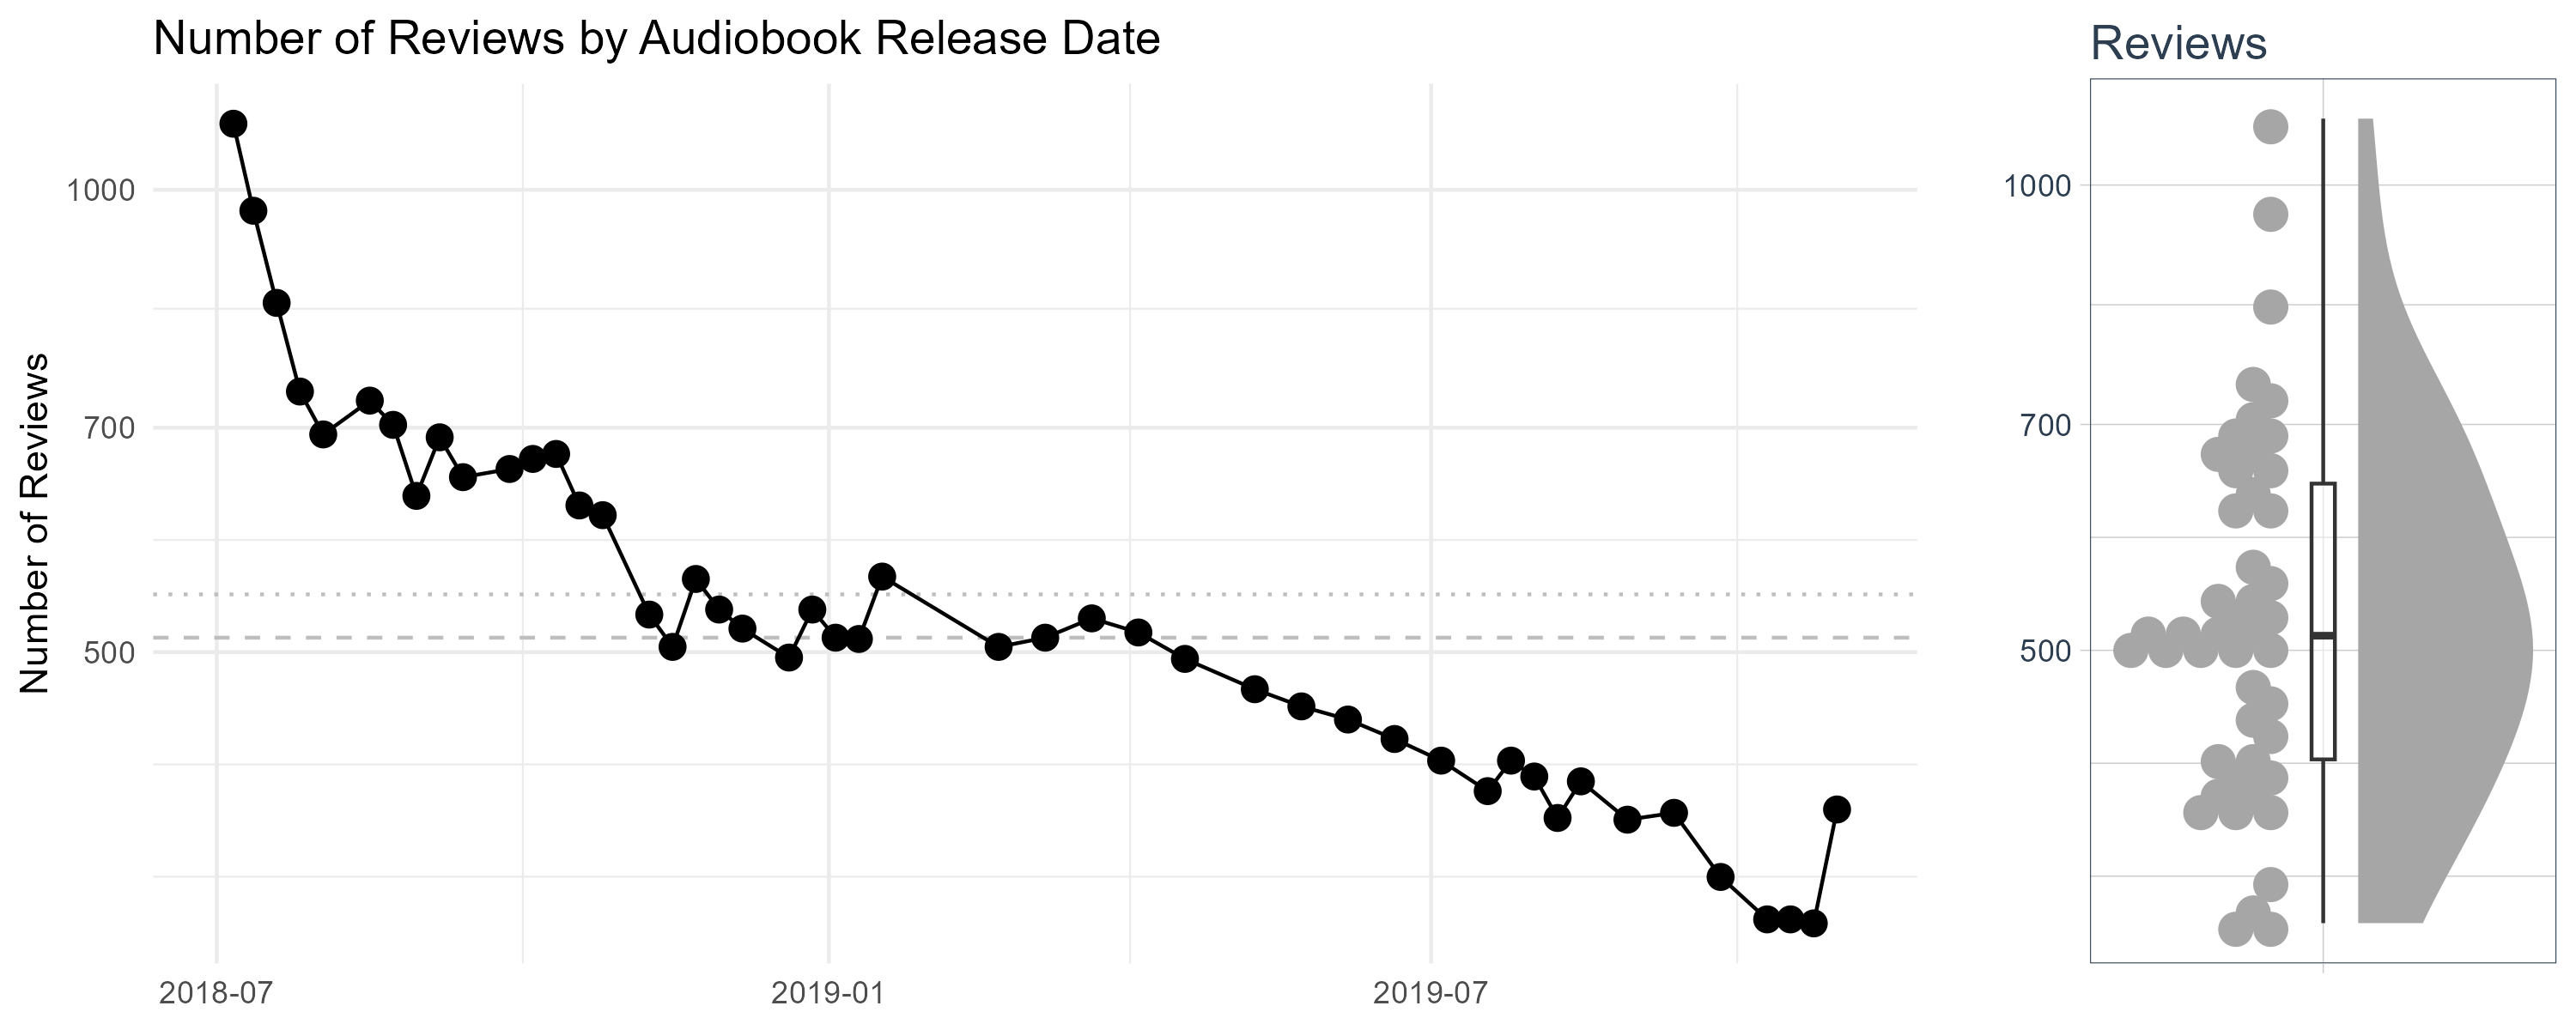
\includegraphics[width=\textwidth]{charts/storytel_reviews}

    The series has a dedicated fanbase, with consistently high engagement, a solid median review count of 511,
    and even the least-reviewed book gathering 333 reviews.

    Releases on Thursdays, spaced 1--2 weeks apart, over 16-months.

\end{frame}

\begin{frame}
    \frametitle{Audiobooks on Storytel: High Ratings}
    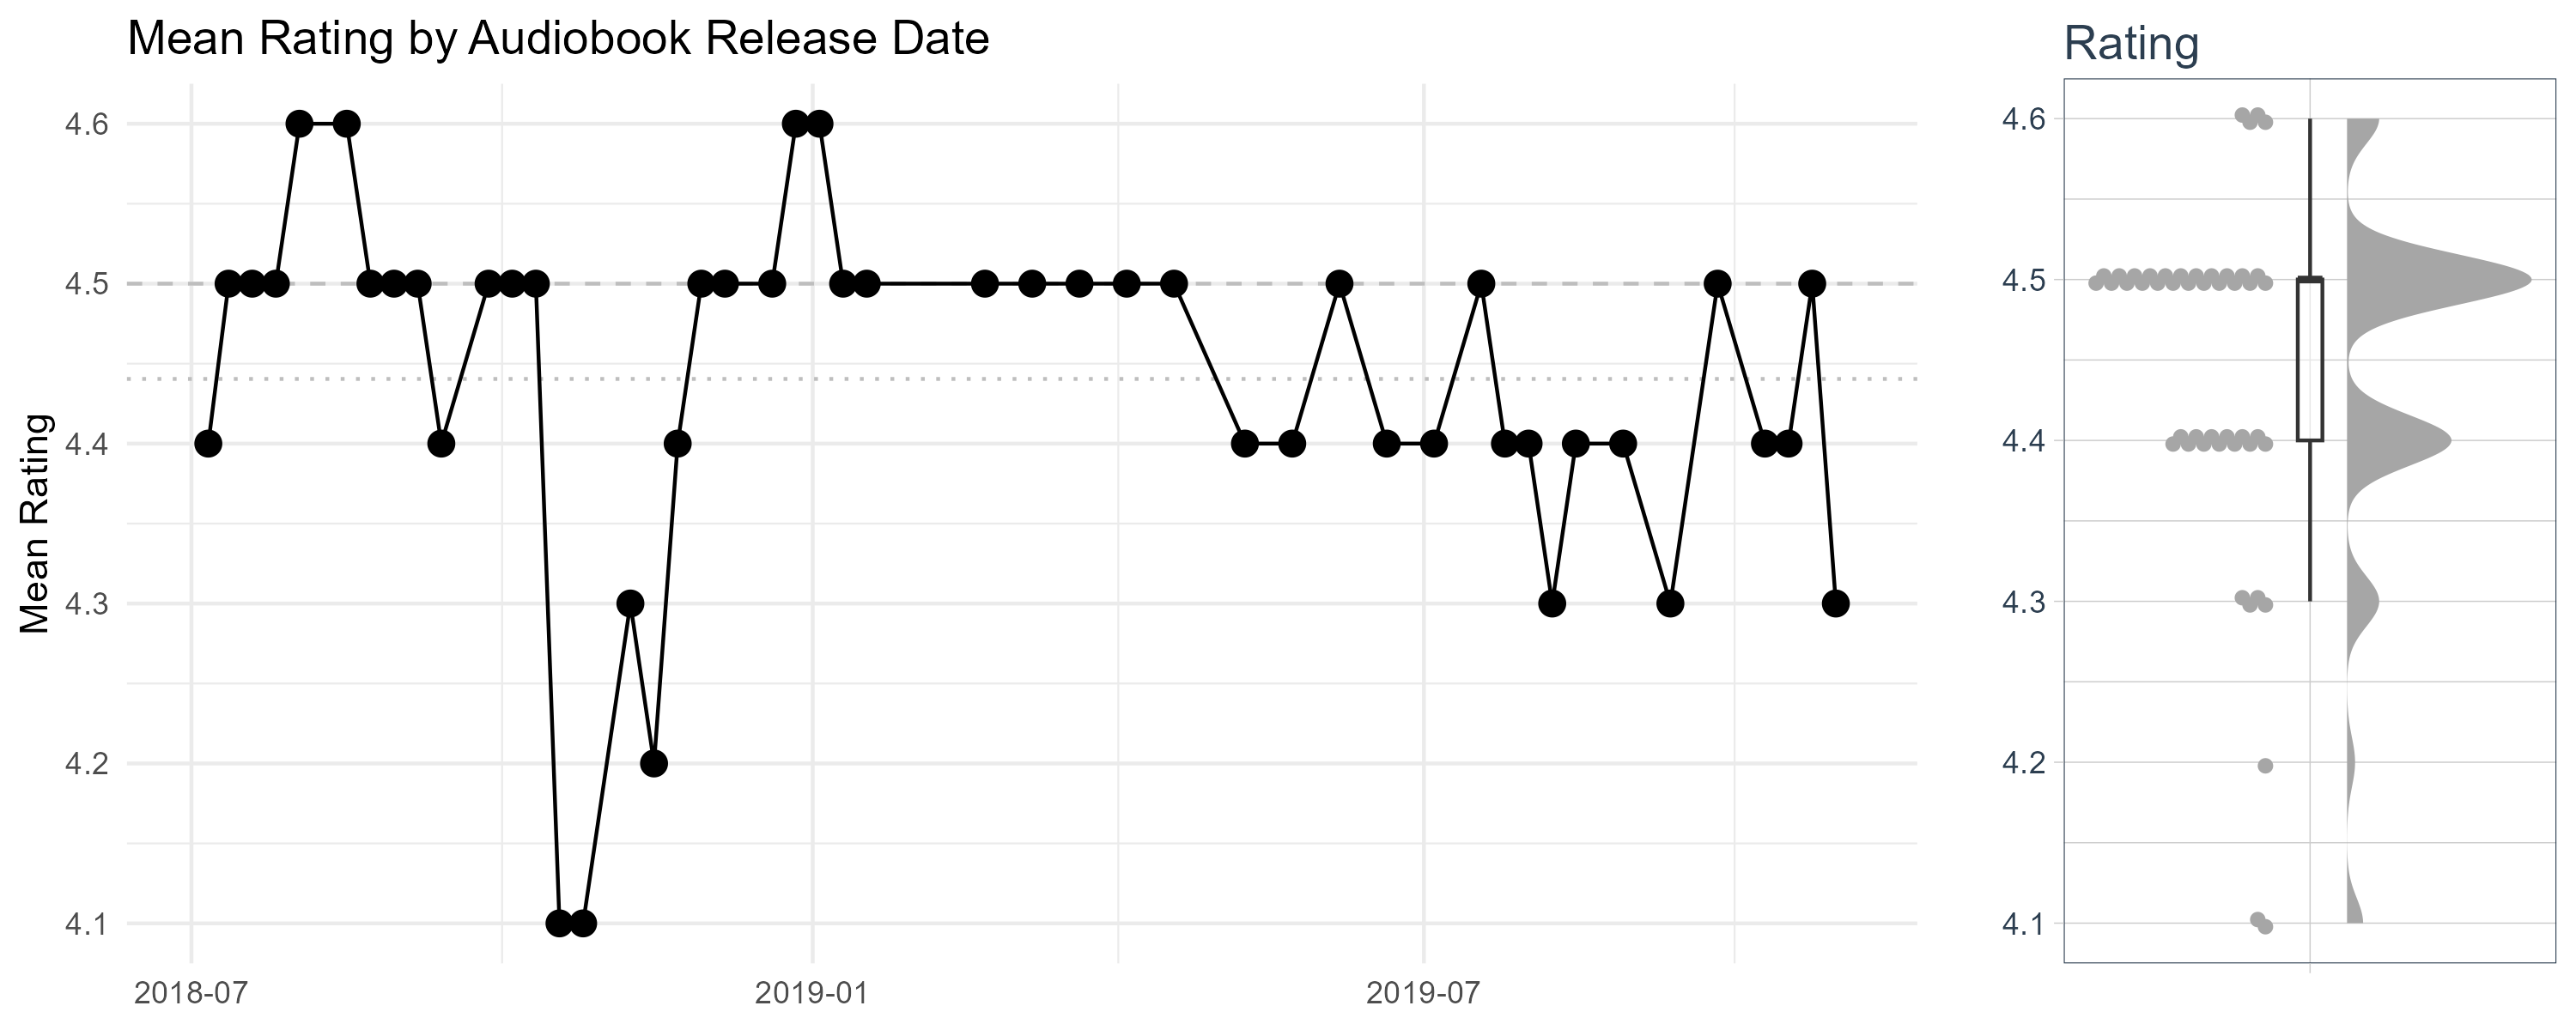
\includegraphics[width=\textwidth]{charts/storytel_ratings}

    Despite a few lower outliers, which can be attributed to a lack of resonance with certain readers and the
    repetitive and slower pace towards the end of the series, the overall rating remains high, with an average
    4.44 stars out of 5.

\end{frame}

\begin{frame}
    \frametitle{Audiobooks on Storytel: Our Narrators}
    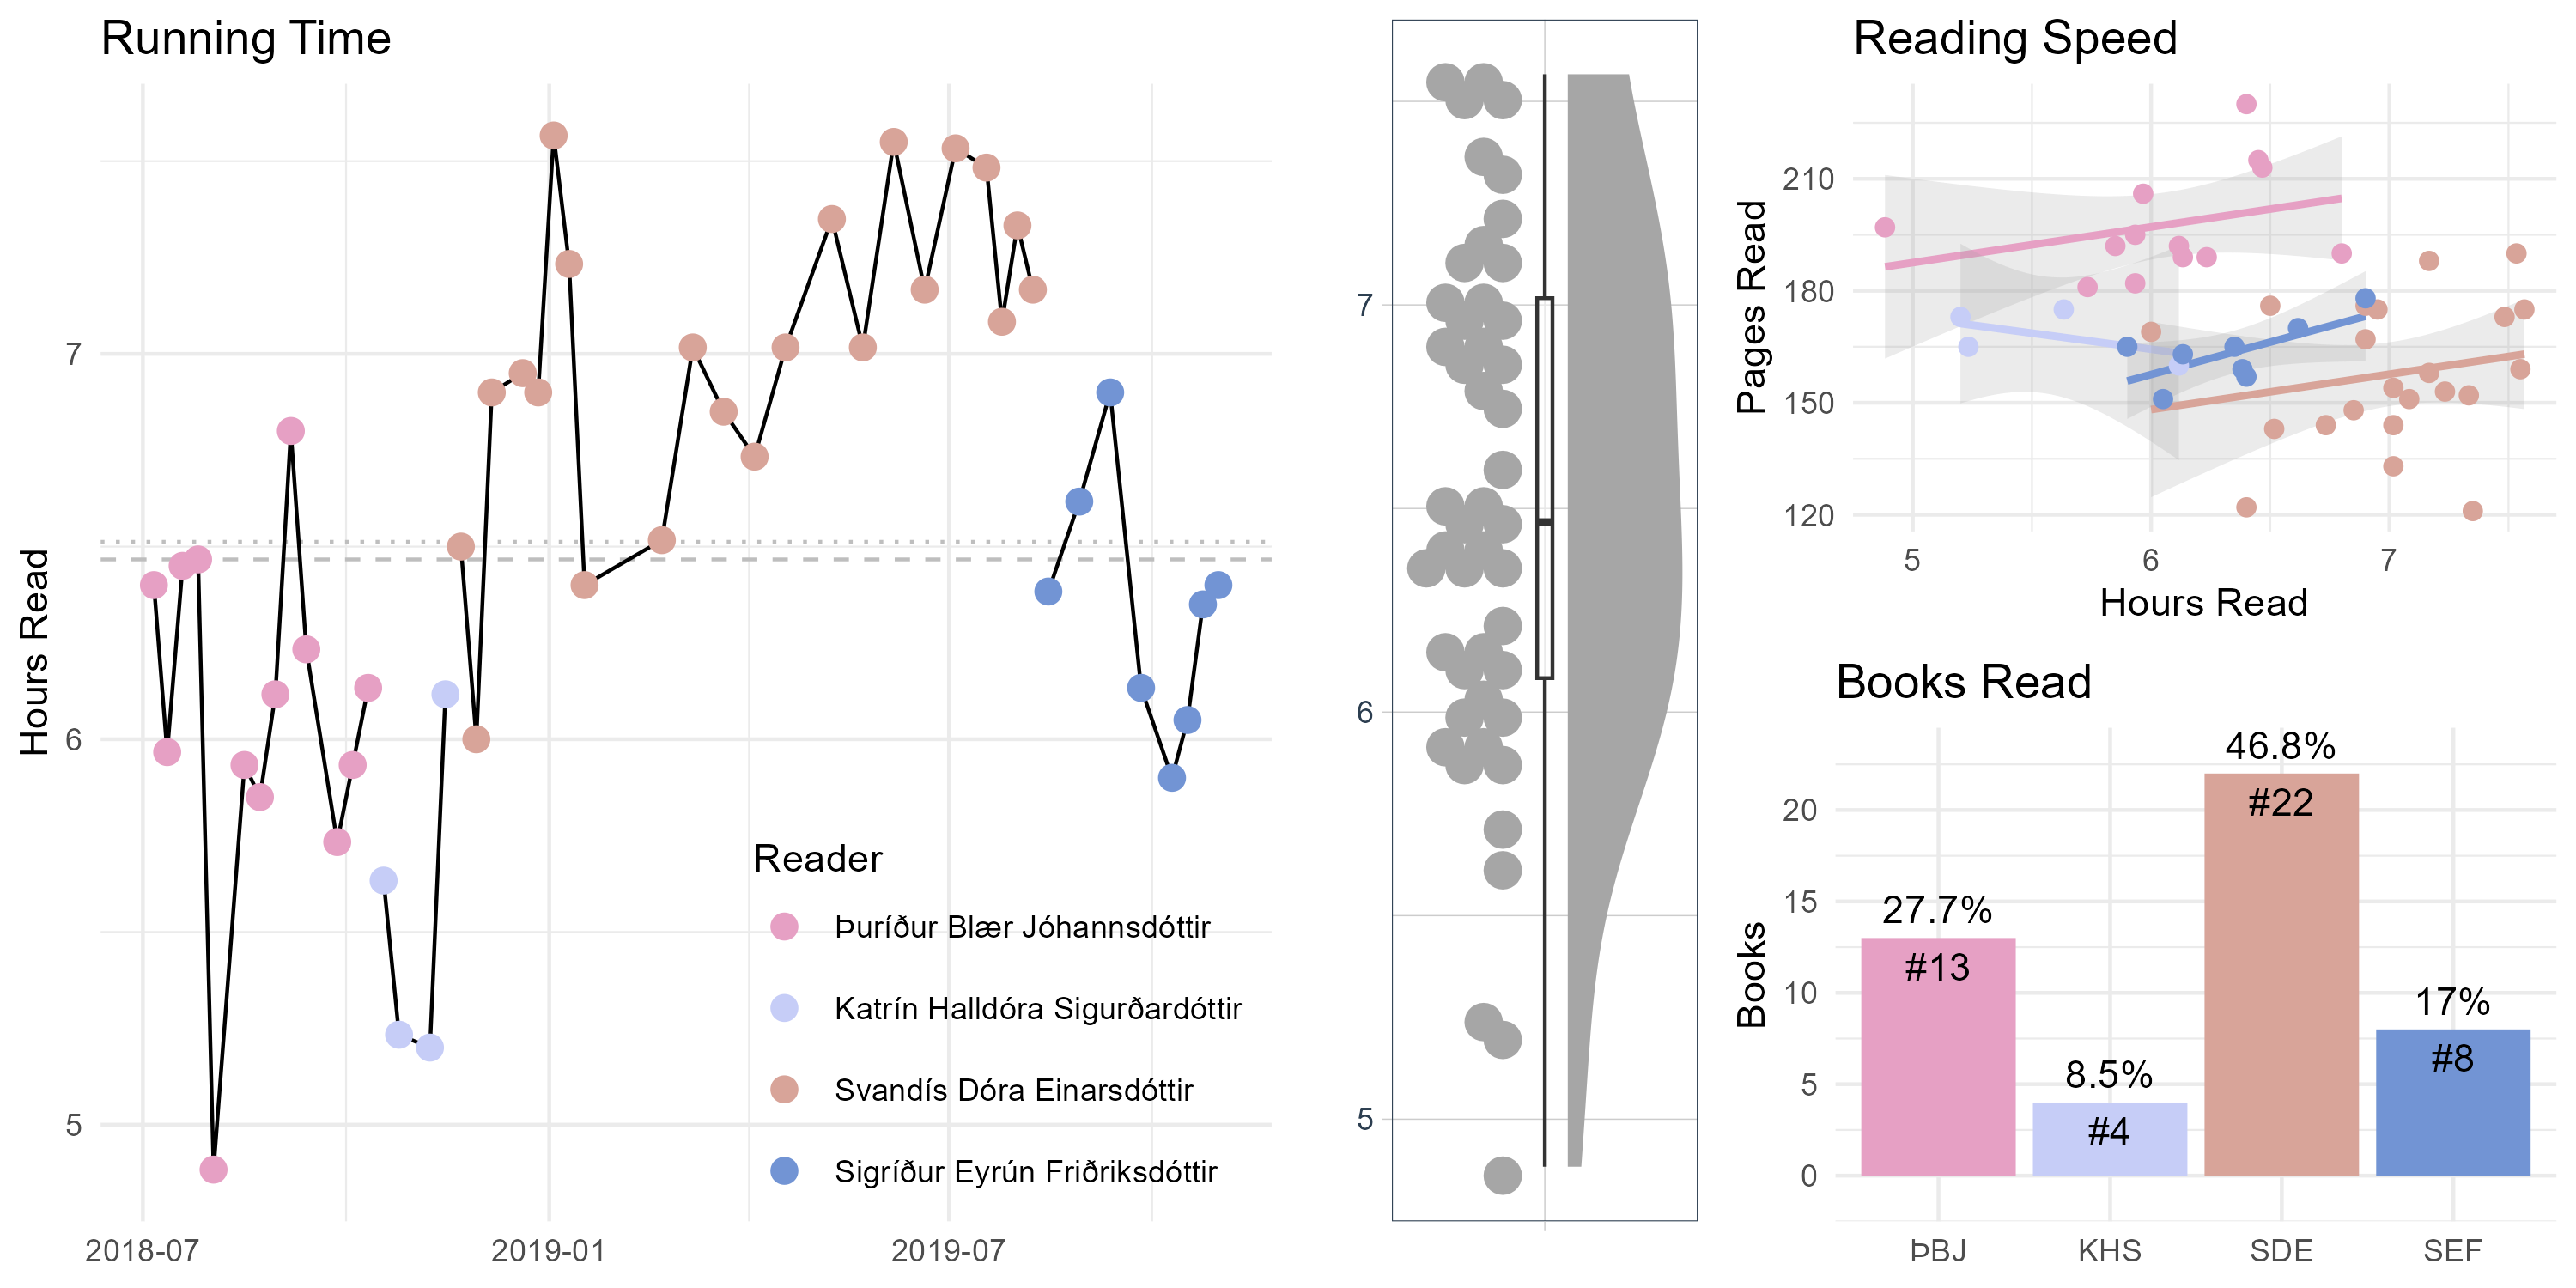
\includegraphics[width=\textwidth]{charts/storytel_readers}
    \vspace{-18pt}
    \begin{itemize}
        \item Over 18K minutes of romantic medieval fantasy -- 12.8 days of continuous listening
        \item Four distinct voices with varied reading styles and perseverance with the series
    \end{itemize}
\end{frame}


\customframe{../rek-data-beers/figures/dalle-podcast}{Podcast}
\begin{frame}{Podcast: Hours Rambled}
    \note{\scriptsize
Moving on, let's discuss the duration of the \emph{ÍSKISUR} podcast episodes available on Alvarpið (a free streaming platform syndicated on Nútíminn.is) and the subscription-based Storytel.

Both platforms introduced the series with a teaser. However, their approaches varied:
\begin{itemize}
    \item Alvarpið had a more freestyle format.
    \item Storytel adhered to a structured approach, ensuring uniform episode durations.
\end{itemize}

The data highlights this: Over 4 years, we produced 7,762 minutes (or 5 days) of content. Episodes on Storytel averaged just under an hour, roughly 10 minutes longer than on Alvarpið. Notably, no episode on either platform exceeded 75 minutes, underscoring our aim for concise, captivating content.
}

    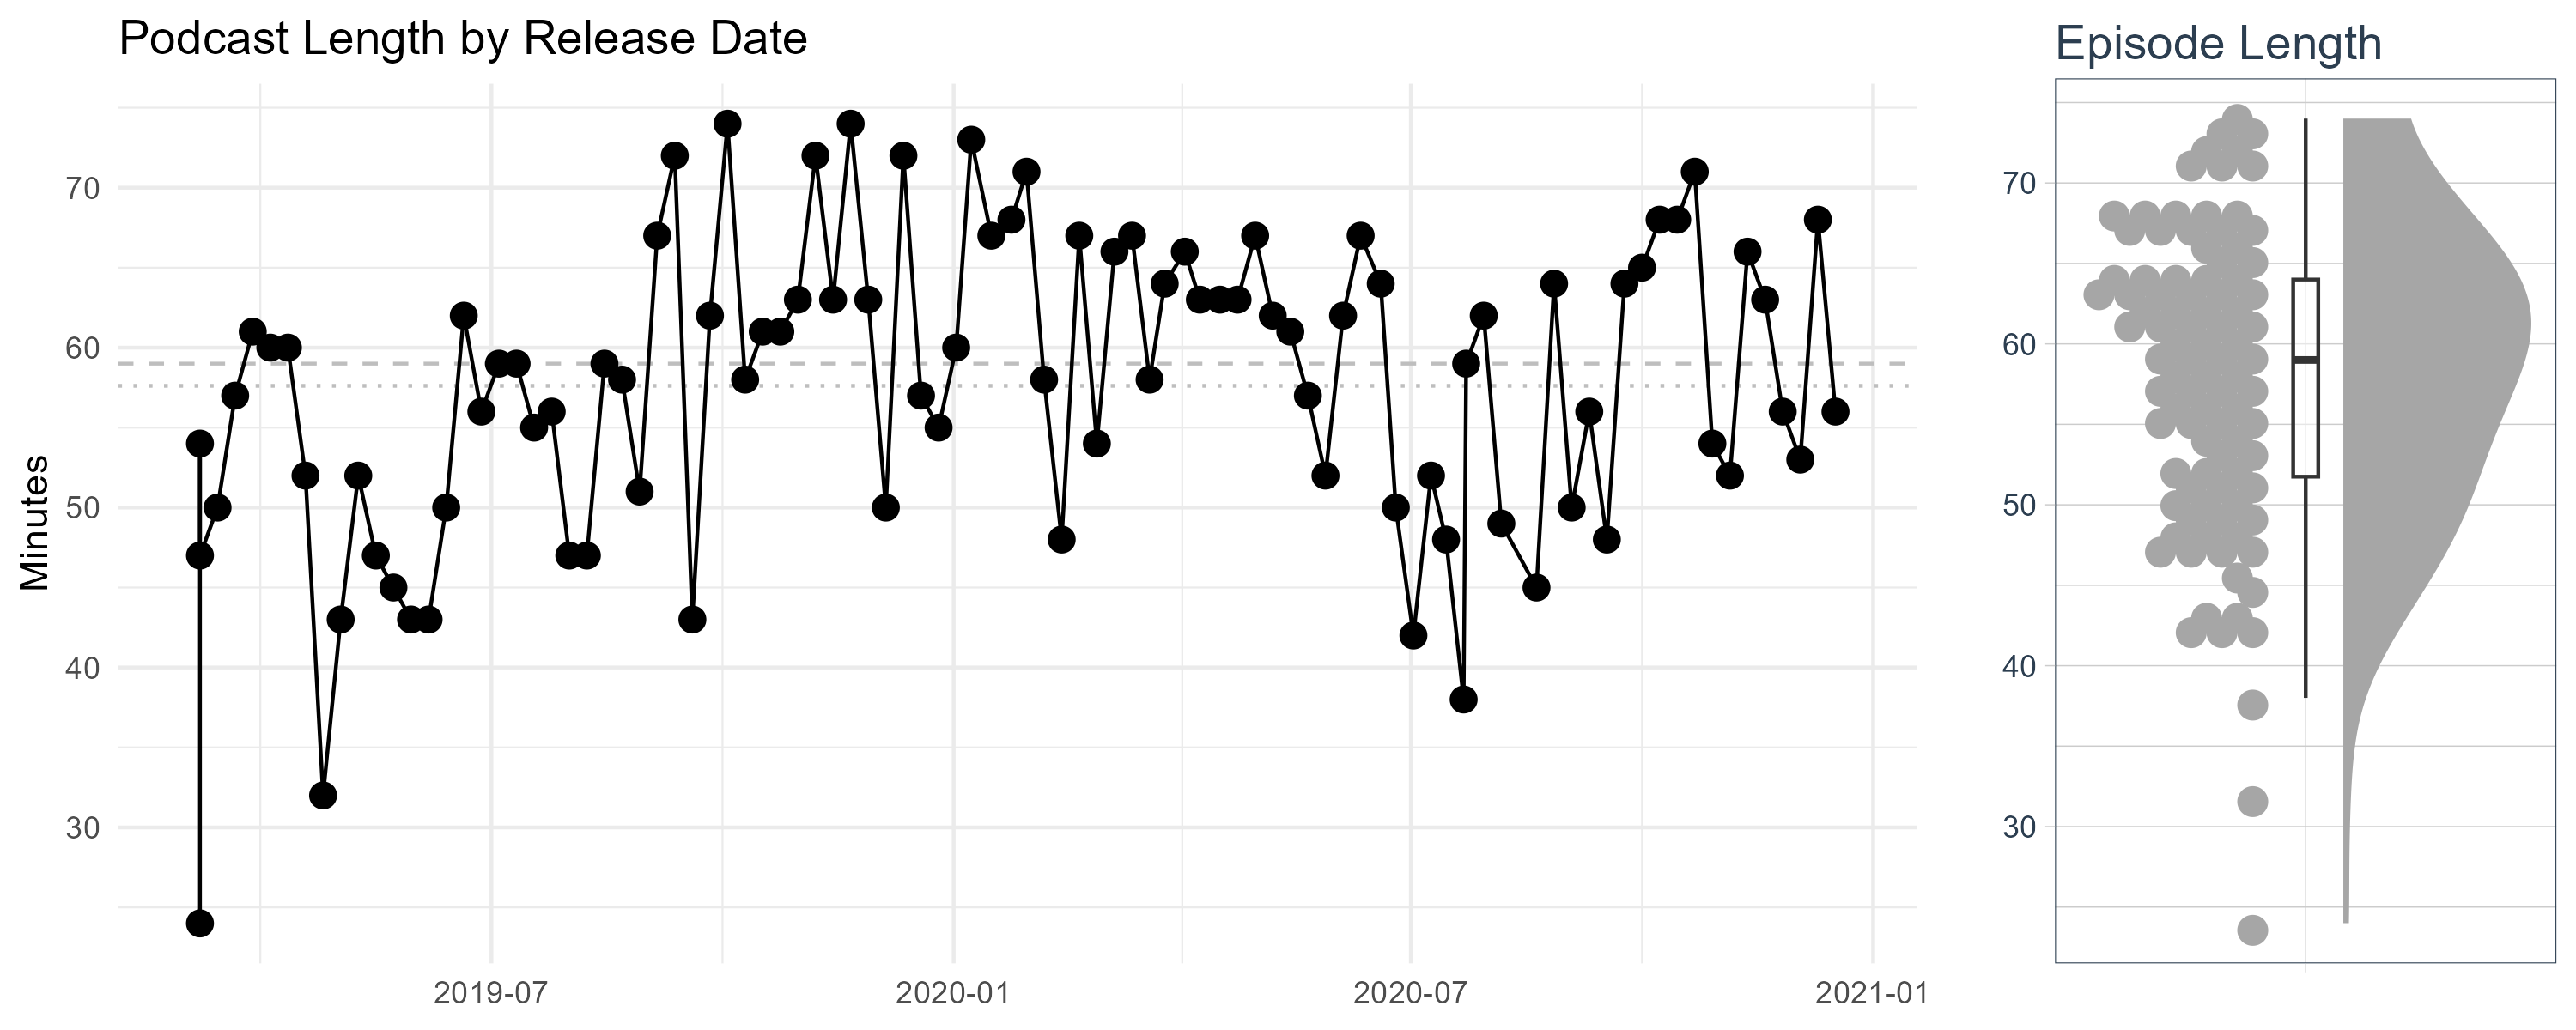
\includegraphics[width=\textwidth]{../R/figures/iskisur_length}
    \begin{itemize}
        \item Over a period of 45.8 months, there is 7,762 minutes of \emph{quality} content, or 5.4 days of continuous
        listening.
        \item Average length is 57.6 minutes on Storytel (48.5 on Alvarpið), but never surpassing 75 minutes.
    \end{itemize}
\end{frame}

\begin{frame}{Podcast on Alvarpið}
\note{
Diving into our experience with the Alvarpið platform: Over 20 months, we crafted 46 episodes, delving into 5.5 books.

\begin{itemize}
    \item Although I couldn't get exact listener counts for each episode, we were informed of a range of \emph{800-1000} listeners per episode through platforms like iTunes.
    Data from \emph{Nútíminn}, via Mixcloud, reflects around 40 streams per episode.
    \item We started with one chapter per episode but quickly transitioned to two chapters for sustainability.
    \item Challenges arose by the sixth book, with health issues and logistical obstacles cutting short our coverage.
    \item Kristín and I recorded from Reykjavík while Birna was in Reyðarfjörður, revealing the hurdles of independent production.
    \item Fortuitously, Storytel approached us. Their entry not only promised compensation but also took over technical aspects, letting us focus on book discussions and my personal favorite: the cat segment.
\end{itemize}
}
    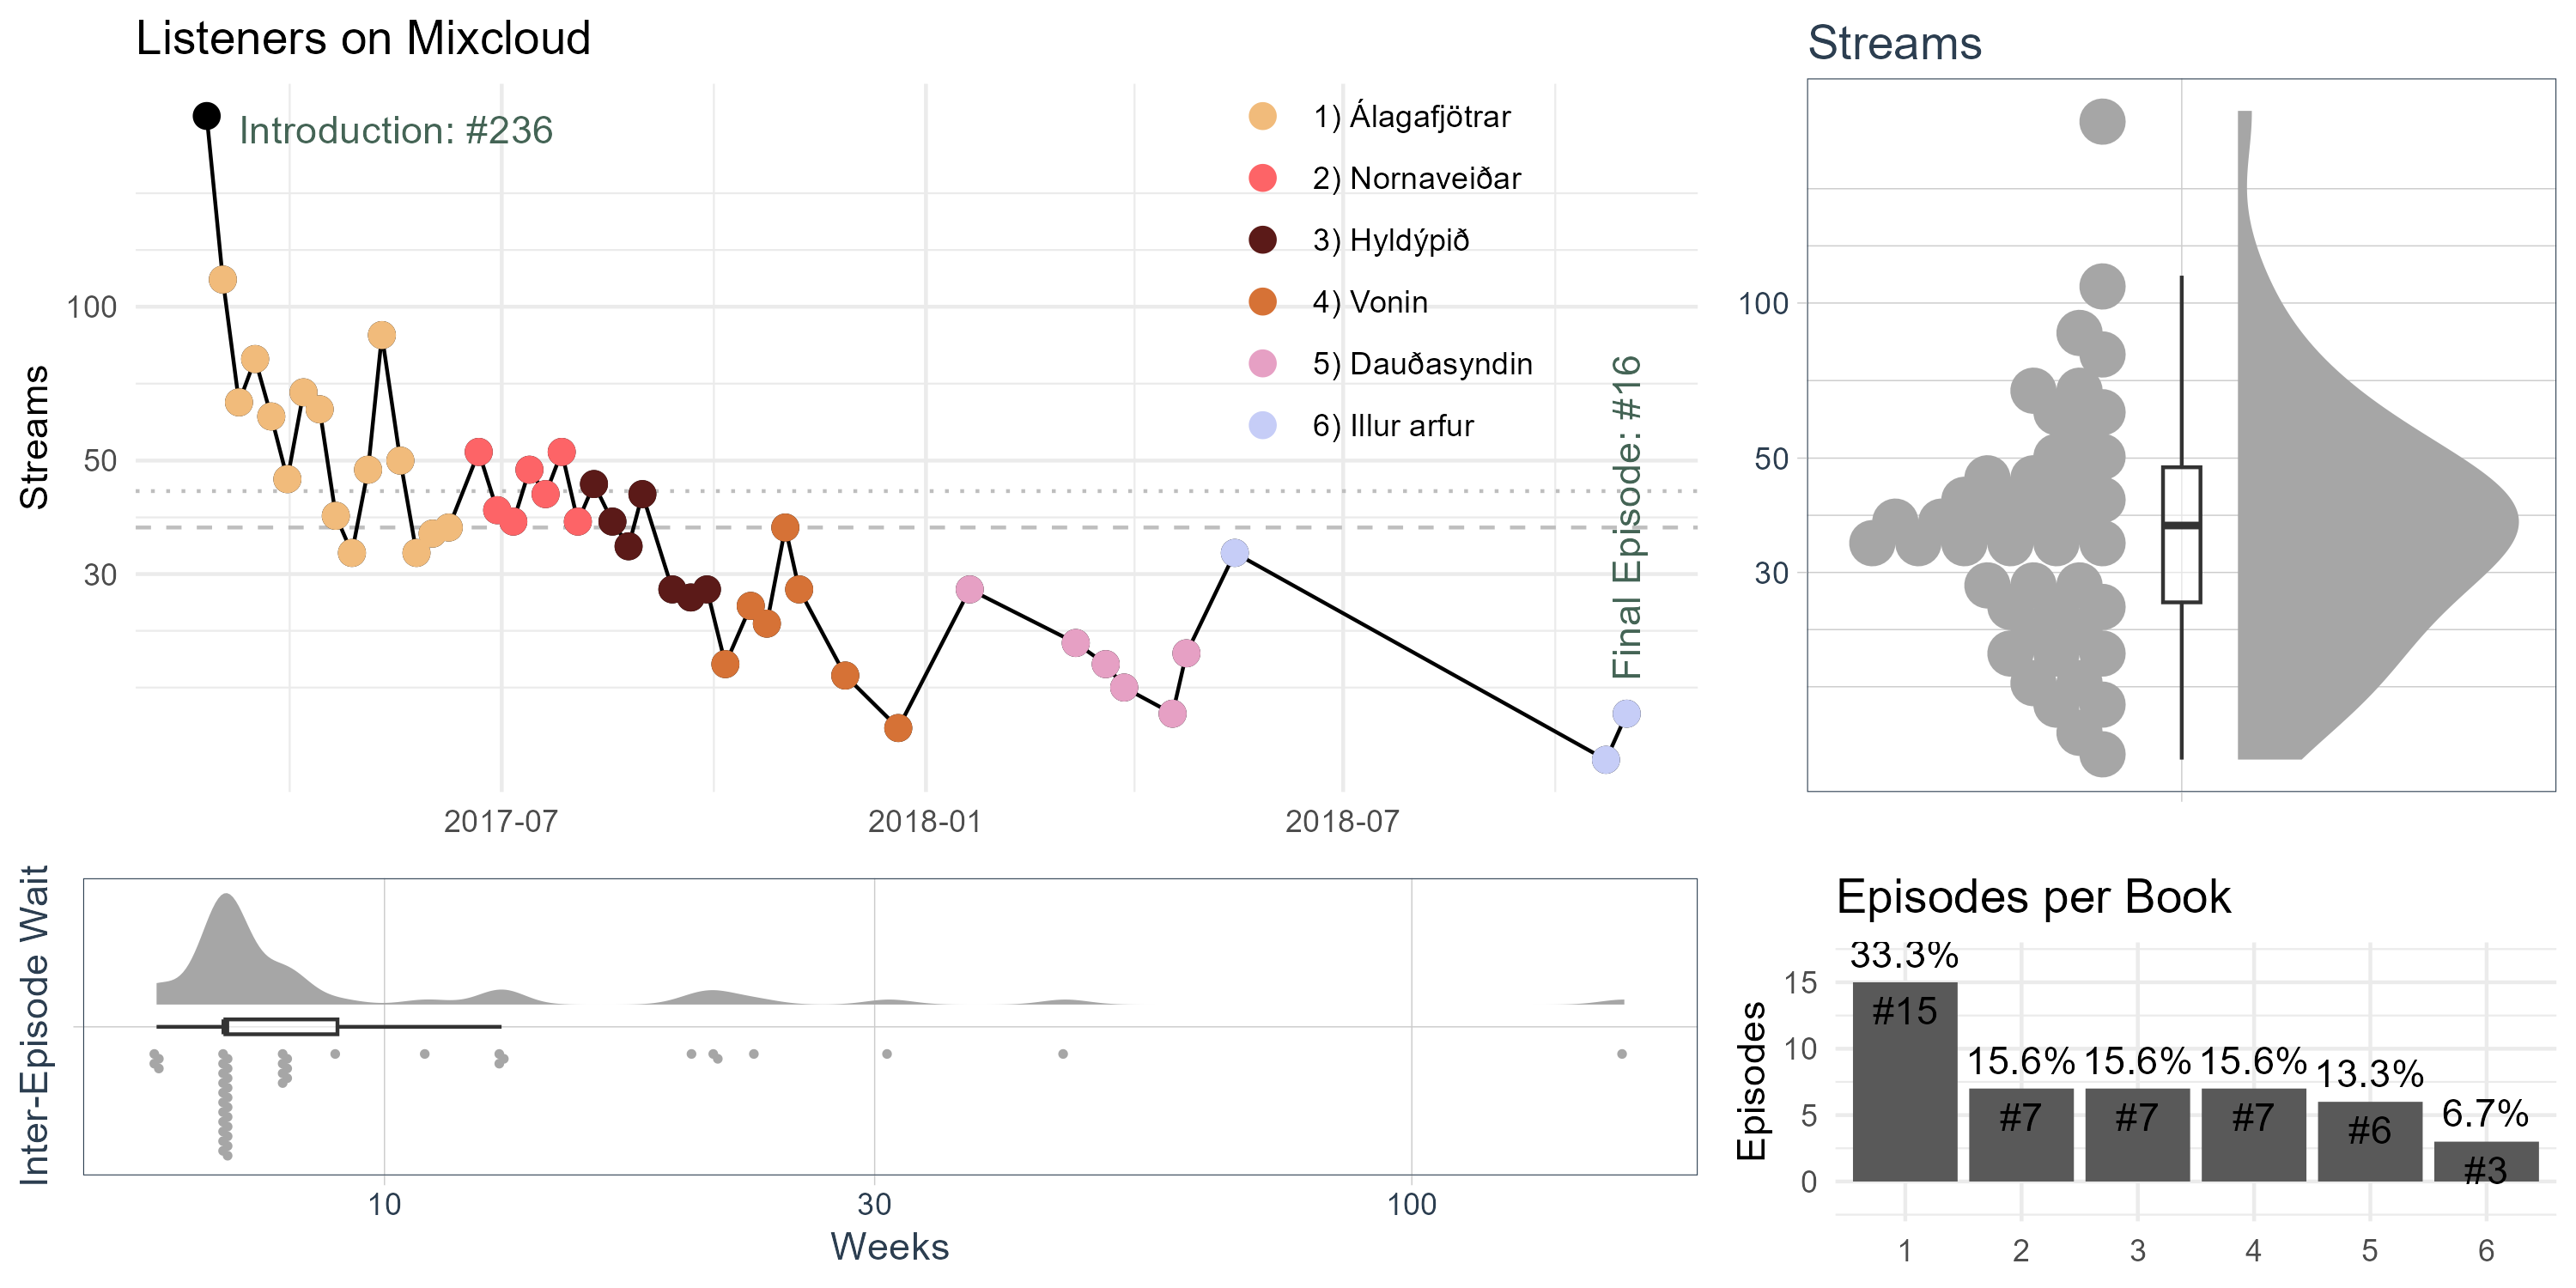
\includegraphics[width=\textwidth]{../R/figures/alvarpid_listeners}
    \vspace{-12pt}
    \begin{itemize}
        \item 46 episodes, 20 months, 5.5 books
        \item 2,231 minutes -- 37 hours -- 1.5 days of continuous listening
        \item Roughly 1,040 streams per episode (thereof ~40 via \url{nutiminn.is})
    \end{itemize}
\end{frame}

\begin{frame}{Podcast on Storytel: High Ratings}
\note{
Teaming up with Storytel brought not just technical relief but also glowing audience feedback, as depicted in this chart.
\begin{itemize}
    \item Our average rating is an outstanding 4.74 out of 5.
    \item Over half of our episodes, 54 to be exact, received a flawless score of 5.0, highlighting listener satisfaction.
    \item Only seven episodes went below a 4.0 rating, with the least score being 3.3.
    \item These figures reflect the consistent quality of our content, augmented by Storytel's professional touch.
\end{itemize}

Switching from the hurdles of Alvarpið's self-production to the streamlined process with Storytel gave our mission renewed vigor.
}
    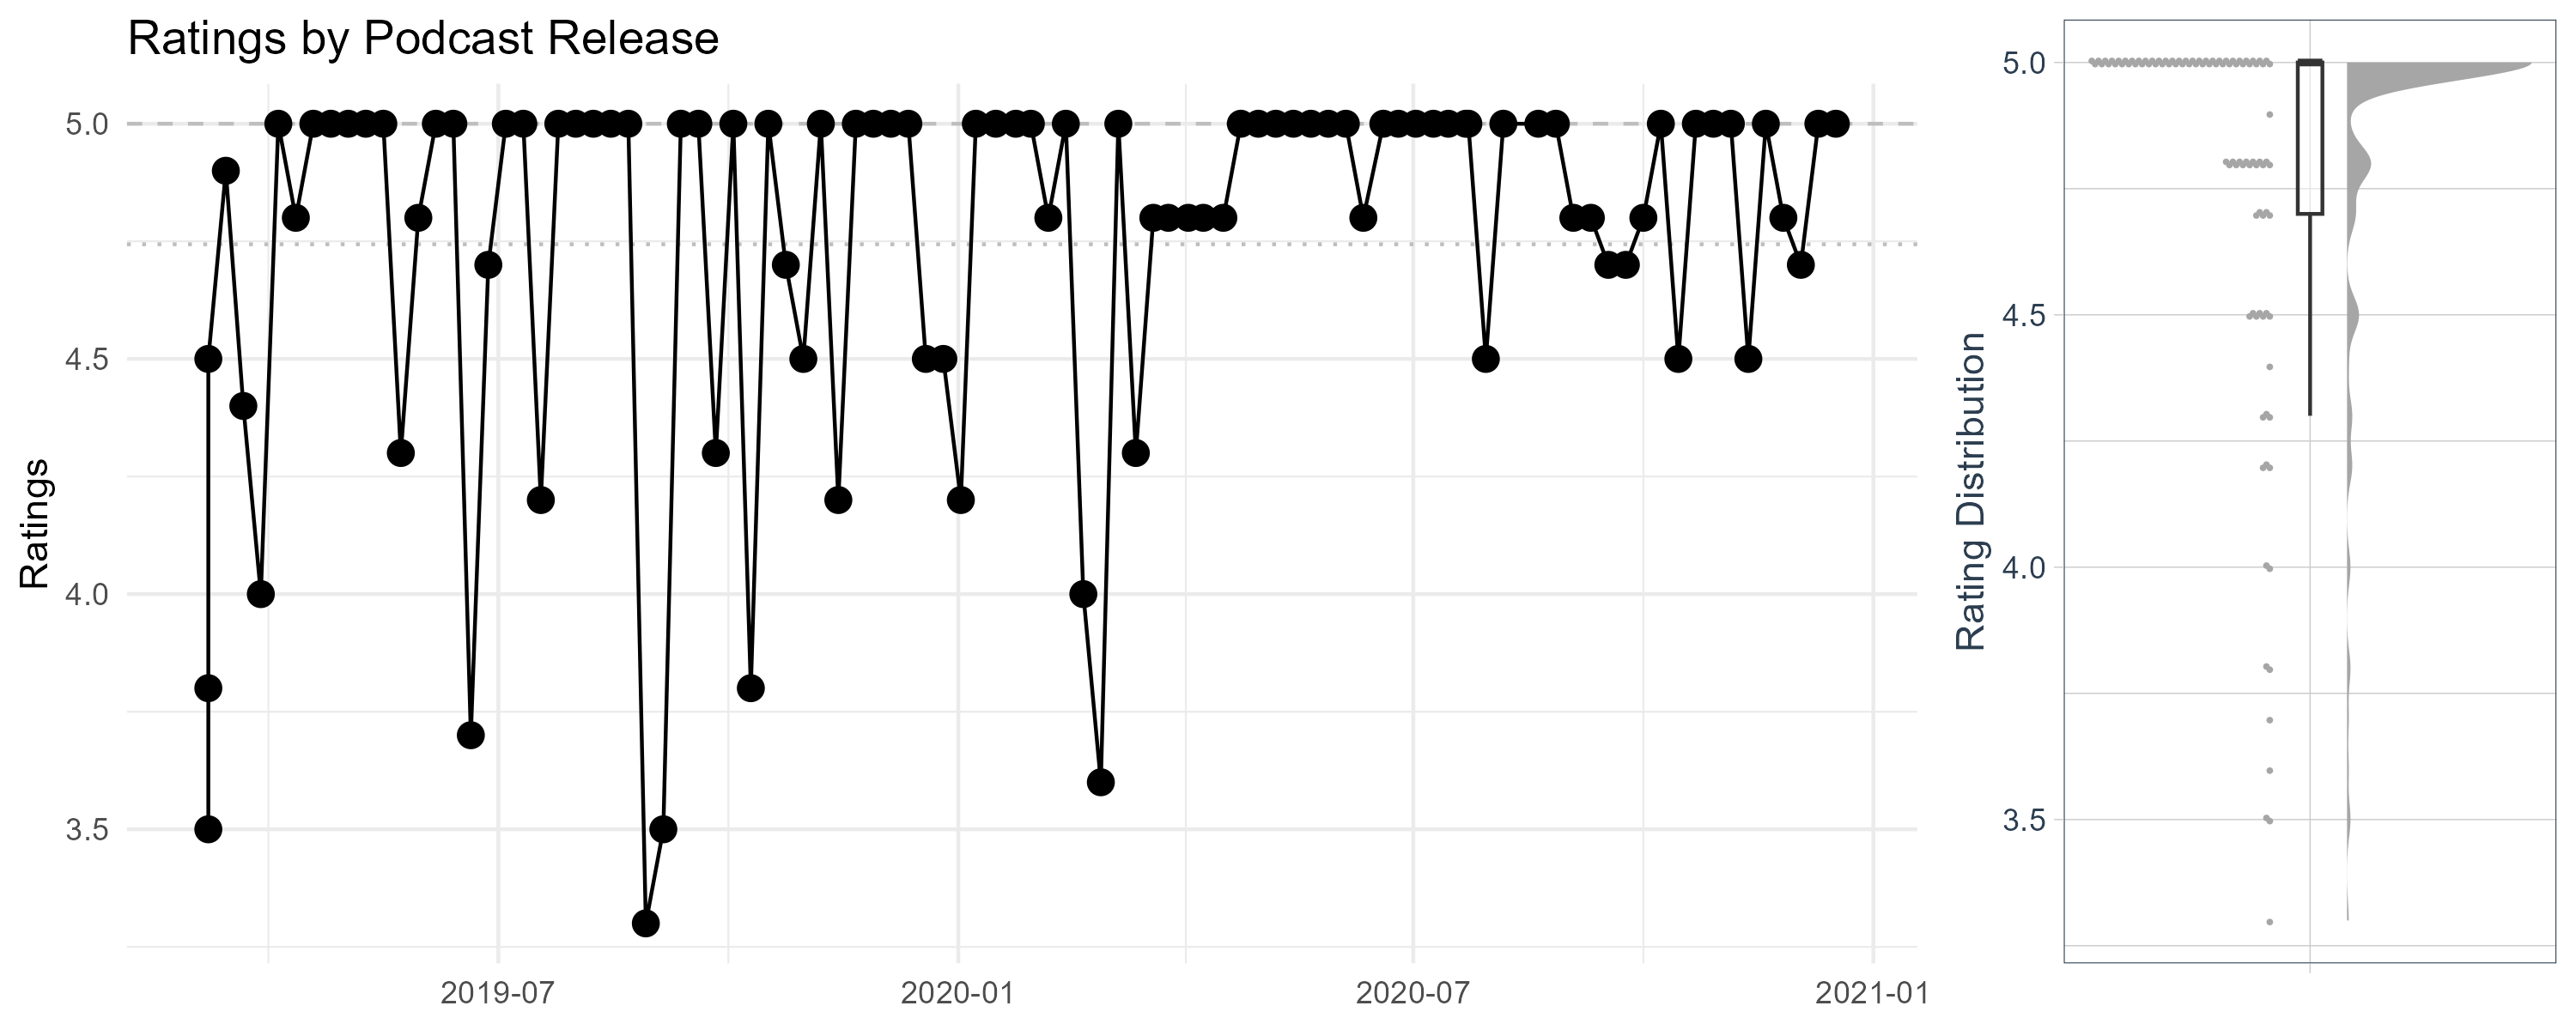
\includegraphics[width=\textwidth]{../R/figures/iskisur_ratings}
    \begin{itemize}
        \item Average rating: 4.74 out of 5
        \item 54 episodes with a perfect 5.0 score (56\% of total)
        \item Only 7 episodes with a rating below 4.0 (worst case 3.3)
    \end{itemize}
\end{frame}

\begin{frame}{Podcast on Storytel: Low Reviews}
\note{\scriptsize

Alright, let's ground ourselves with a touch of humility here.
    Taking a look at this chart, we can see a humbling snapshot: our review count isn't quite as jaw-dropping as we might have hoped.
    Sure, we've got a commendable rating, but in terms of review numbers?
    Our 444 reviews are dwarfed by the 25,627 the audiobooks received.
    Clearly, we were a small fish in the Storytel pond.

    \emph{Full disclosure}: I didn't religiously review our podcast episodes.
    After the initial rush of hearing our voices on the platform, I realized that since I was relistening during post-processing
    (penning the accompanied text summaries – a must-read, by the way), there wasn't much point in re-re-relistening.
    I've believe my co-hosts shared my sentiment.

    However, every silver lining has its cloud:
    \begin{itemize}
        \item We always had at least \emph{one} die-hard fan who never failed to review,
        \item and we'll forever be grateful to those \emph{four} mainstays who consistently showered us with feedback.
    \end{itemize}

    While our podcast felt like a cozy book club, a running joke was that there was only one listener.
    But looking at our review count, it seems the joke was closer to the truth than we thought.
    Nonetheless, it's not the quantity that matters, but the quality.

}
    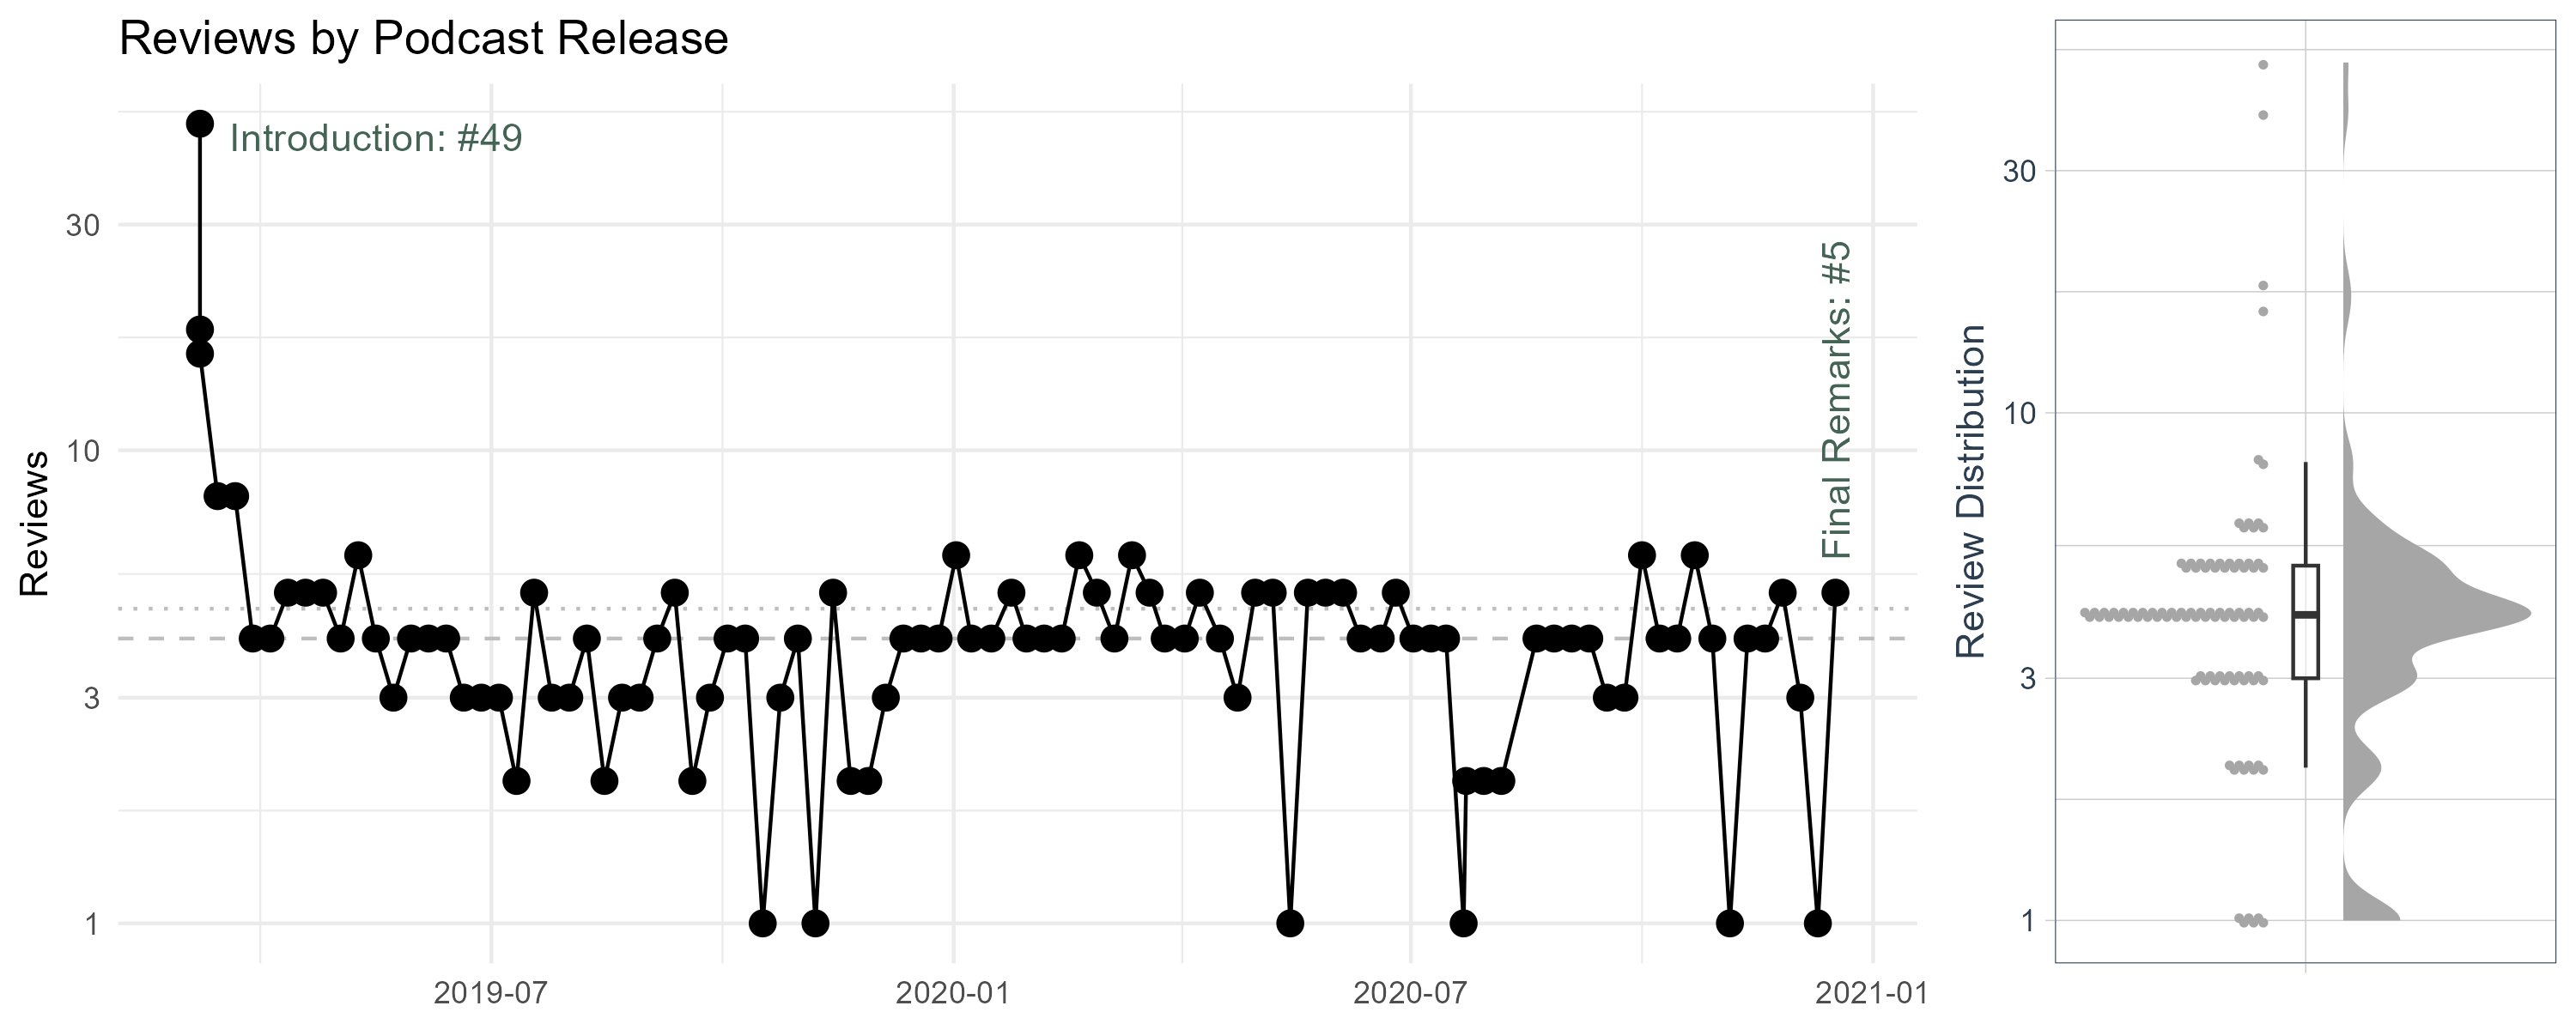
\includegraphics[width=\textwidth]{../R/figures/iskisur_reviews}
    \begin{itemize}
        \item Number of reviews: 444 total (25,627 for the audiobooks)
        \item At least one active fan throughout the period
        \item Four regular fans who consistently provided review
    \end{itemize}
\end{frame}

\begin{frame}{Podcast Platform Comparison}
    \note{
    As we conclude, here's a bird's-eye view of our podcast journey:
    \begin{itemize}
        \item We went from crafting 46 episodes on Alvarpið to a staggering 96 on Storytel.

        \item The average episode length slightly increased on Storytel.

        \item Notice the stark difference in release consistency: Alvarpið saw gaps as long as 161 days, while Storytel never went beyond a 14-day hiatus.

        \item In terms of overall engagement, both platforms gave us roughly 20 months of active podcasting each, but let's not forget that 4.1-month pause we took in between.
    \end{itemize}

    Most importantly, we had a blast throughout the journey, and we managed to cover all 47 books in the series in record time (in true Margit fashion)
    }
    \begin{table}[]
        \begin{tabular}{l|rr|rr|rrr|r}
            & \rotatebox{90}{Episodes} & \rotatebox{90}{Books} &
            \rotatebox{90}{Total Running Time (hours)} & \rotatebox{90}{Average Length (min)} &
            \rotatebox{90}{Median Days to Next}
            & \rotatebox{90}{Average Days to Next}  & \rotatebox{90}{Max Days to Next}  &
            \rotatebox{90}{Months Active} \\
            \midrule
            Alvarpið & 46  & 6  & 37.2  & 48.50 & 7 & 13.69 & 161 & 20.3  \\
            Storytel & 96  & 47 & 92.2  & 57.61 & 7 & 6.85  & 14  & 21.4  \\
            \midrule
            & 142 &    & 129.4 &       &   &       &     & 45.8*
        \end{tabular}
    \end{table}

    \vfill
    \footnotesize{*4.1 months hiatus between Alvarpið and Storytel}
\end{frame}


\customframe{../rek-data-beers/figures/dalle-book-6}{Storyline}
\begin{frame}{Ice People Family Tree}
    \note{\scriptsize
    \begin{itemize}

        \item Diving into the narrative intricacies of the 47-book saga,
        we're brought face-to-face with a sprawling family tree that traces its lineage
        back to the matriarch Silja Arngrímsdóttir and her cursed beau, Þengill the good.

        \item Their descendants' tangled relationships are laid out here,
        and it's impossible to ignore the density of the connections --
        hinting at a significant amount of inbreeding.
        This compact lineage, while perhaps challenging for readers (and narrators!)
        to digest given its incestuous undertones, does offer us a silver lining --
        it's surprisingly \emph{slide-friendly}. Managing to represent 17 generations in one visual
        would generally be a challenge, but this is a rare exception.

        \item Cursed family members are color-coded: yellow for \emph{virtuous}, green for \emph{malevolent}, and pink for those who found \emph{redemption}.

        \item As we scan through the tree, it's curious to note that the distribution of the curse
        doesn't seem to follow a strict genetic pattern. Entire generations sometimes escape its grasp,
        suggesting that Margit perhaps allowed a degree of creative freedom over genetic accuracy in
        deciding who bears the curse.

        \item This intricate web of relationships, filled with cursed figures,
        highlights the need for a data-driven approach to unravel and understand Margit's artistic choices.
        \end{itemize}
}
    \centering
    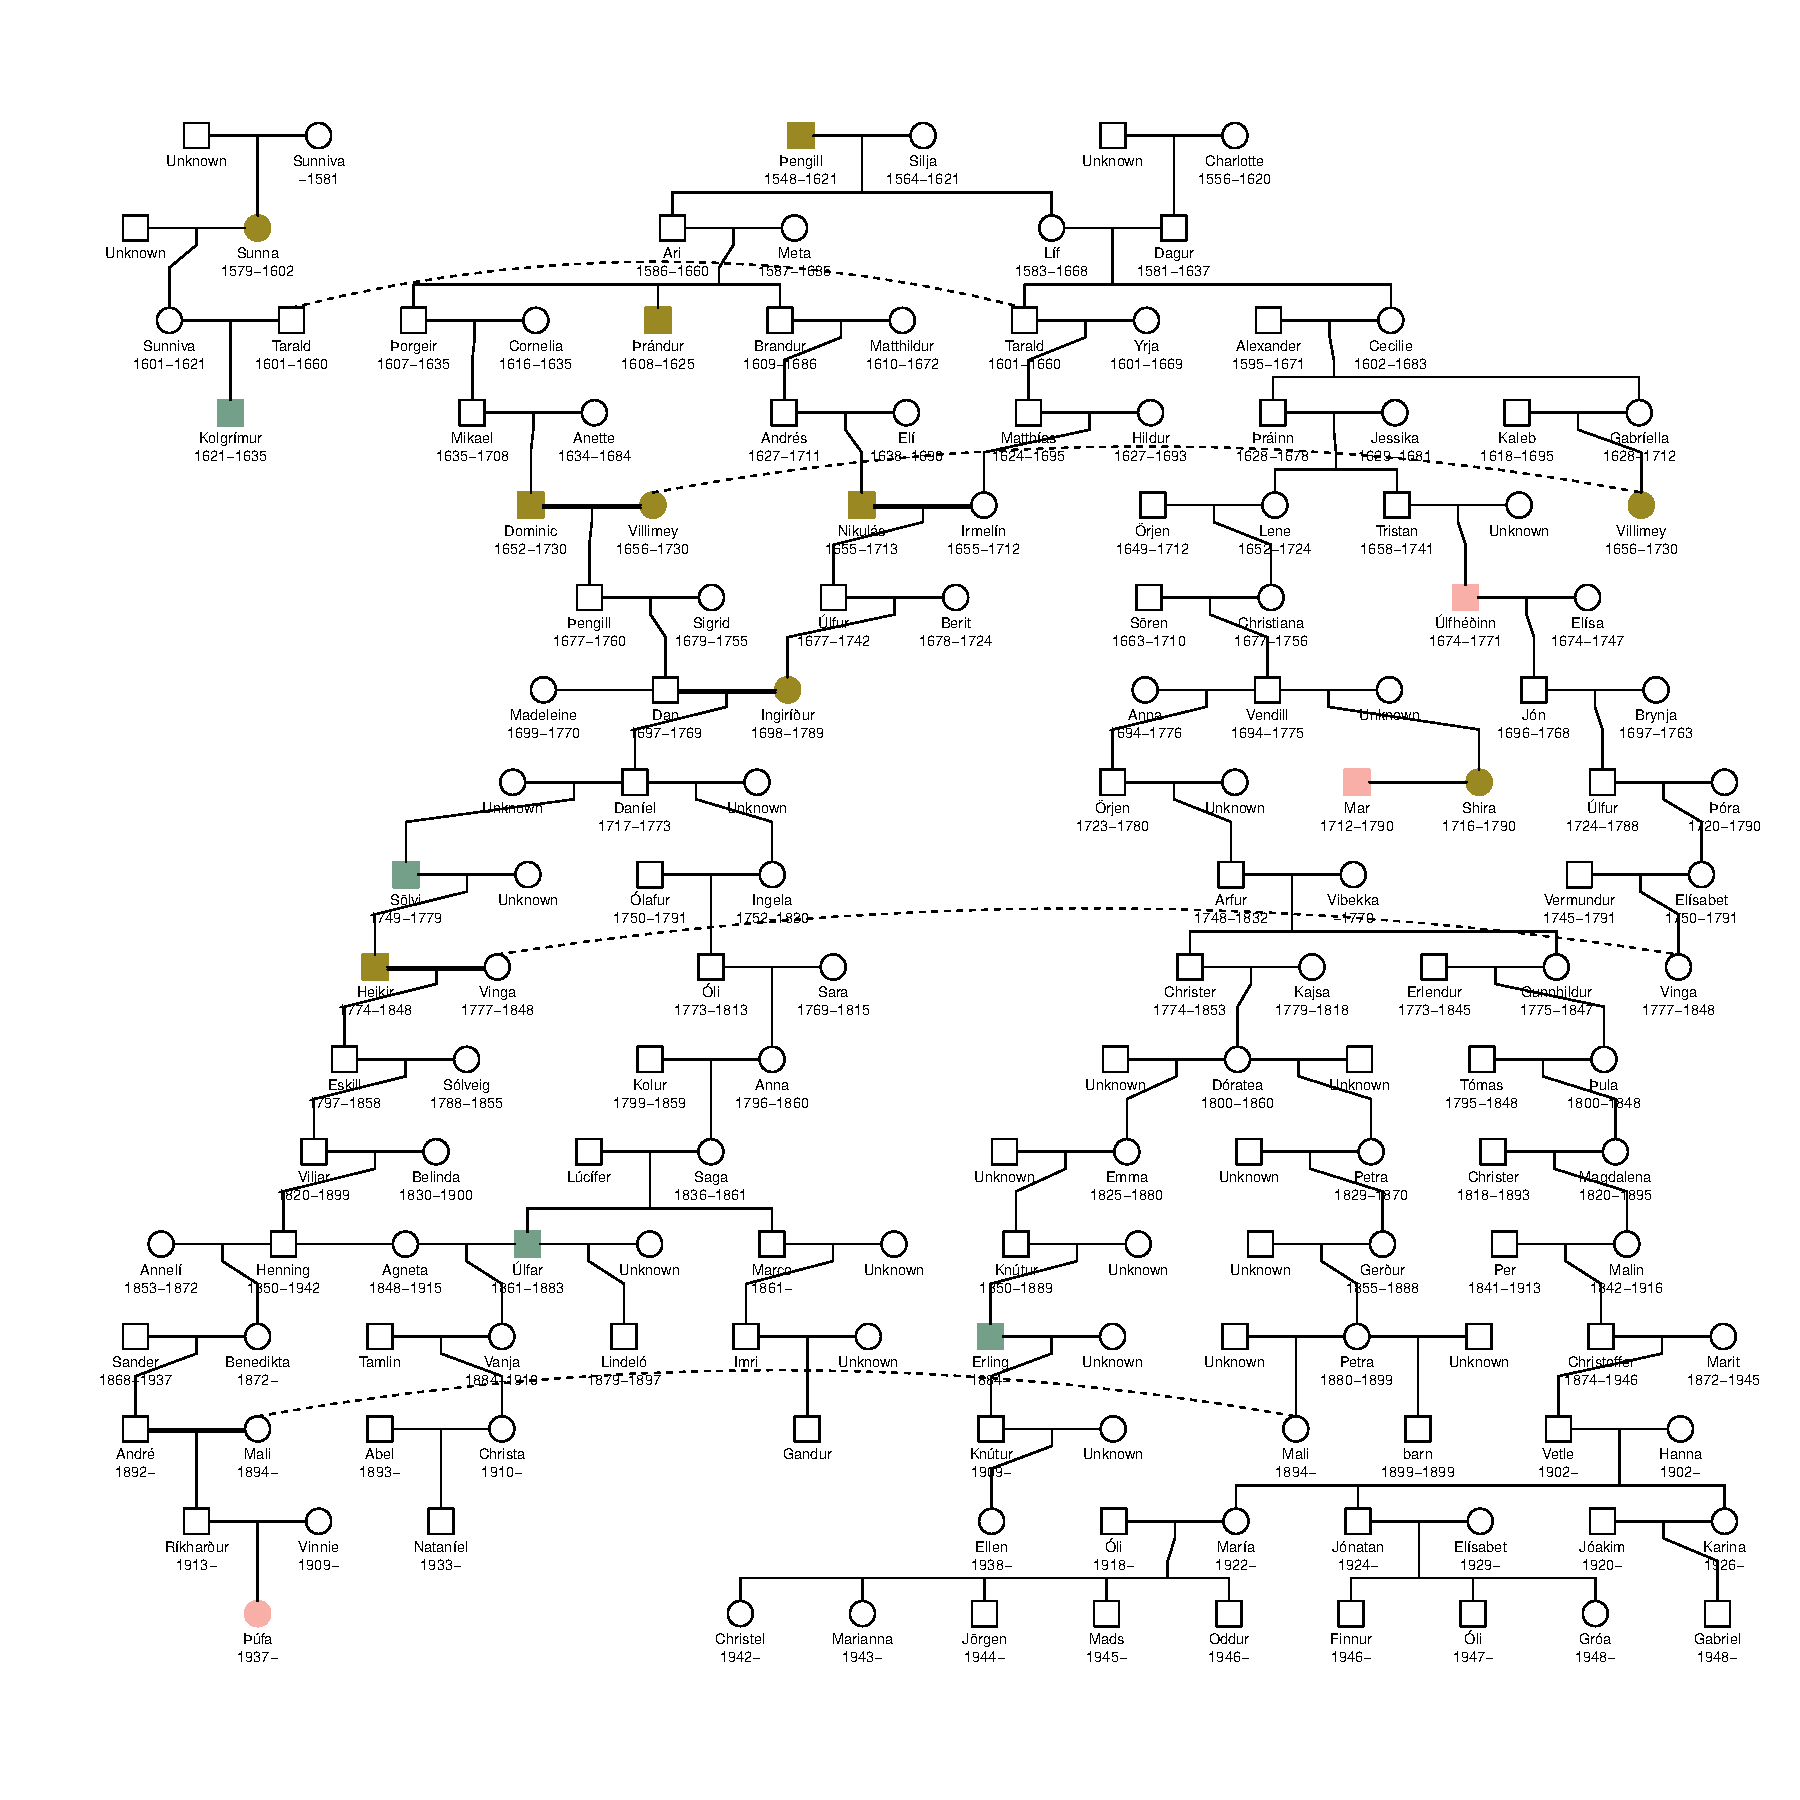
\includegraphics[height=.9\textheight]{../R/figures/family_tree}
\end{frame}

\begin{frame}{Ice People Family Gantt Chart}
    \note{\scriptsize
    \begin{itemize}
        \item To decipher the complex family tree and its concurrent relationships,
        we turned to a \emph{data transformation}: the \emph{Gantt} chart,
        usually a tool for project timelines, but here, it's a brilliant
        visualization of lifespans and intersecting narratives.

        \item Spanning from the mid-1600s to the 1960s, this chart offers clear insights
        into overlapping lifetimes, painting a vivid picture of contemporaneous
        characters.

        \item Margit frequently intertwines character narratives,
        often through romantic unions. This attraction amongst cousins is
        both a narrative device and a manifestation of their shared, cursed lineage.
        Despite many generations, the family size stays around 20 members, peaking at 30 later on.

        \item Typically, 1-2 cursed individuals from the Ice People are alive at any given time. However, a spike occurs in the early 1700s with six simultaneous cursed beings.
        \item Mar, in particular, isn't directly of the Ice People. He's of the Taranqyes lineage, which traces back to their common ancestor the infamous Þengill the Bad.
        \item The gaps in the family tree regarding cursed individuals suggest that the Taranqyes lineage might be the ones carrying the curse for those missing generations, as the narrative asserts there's always one cursed person per generation.
        \end{itemize}
    }
    \centering
    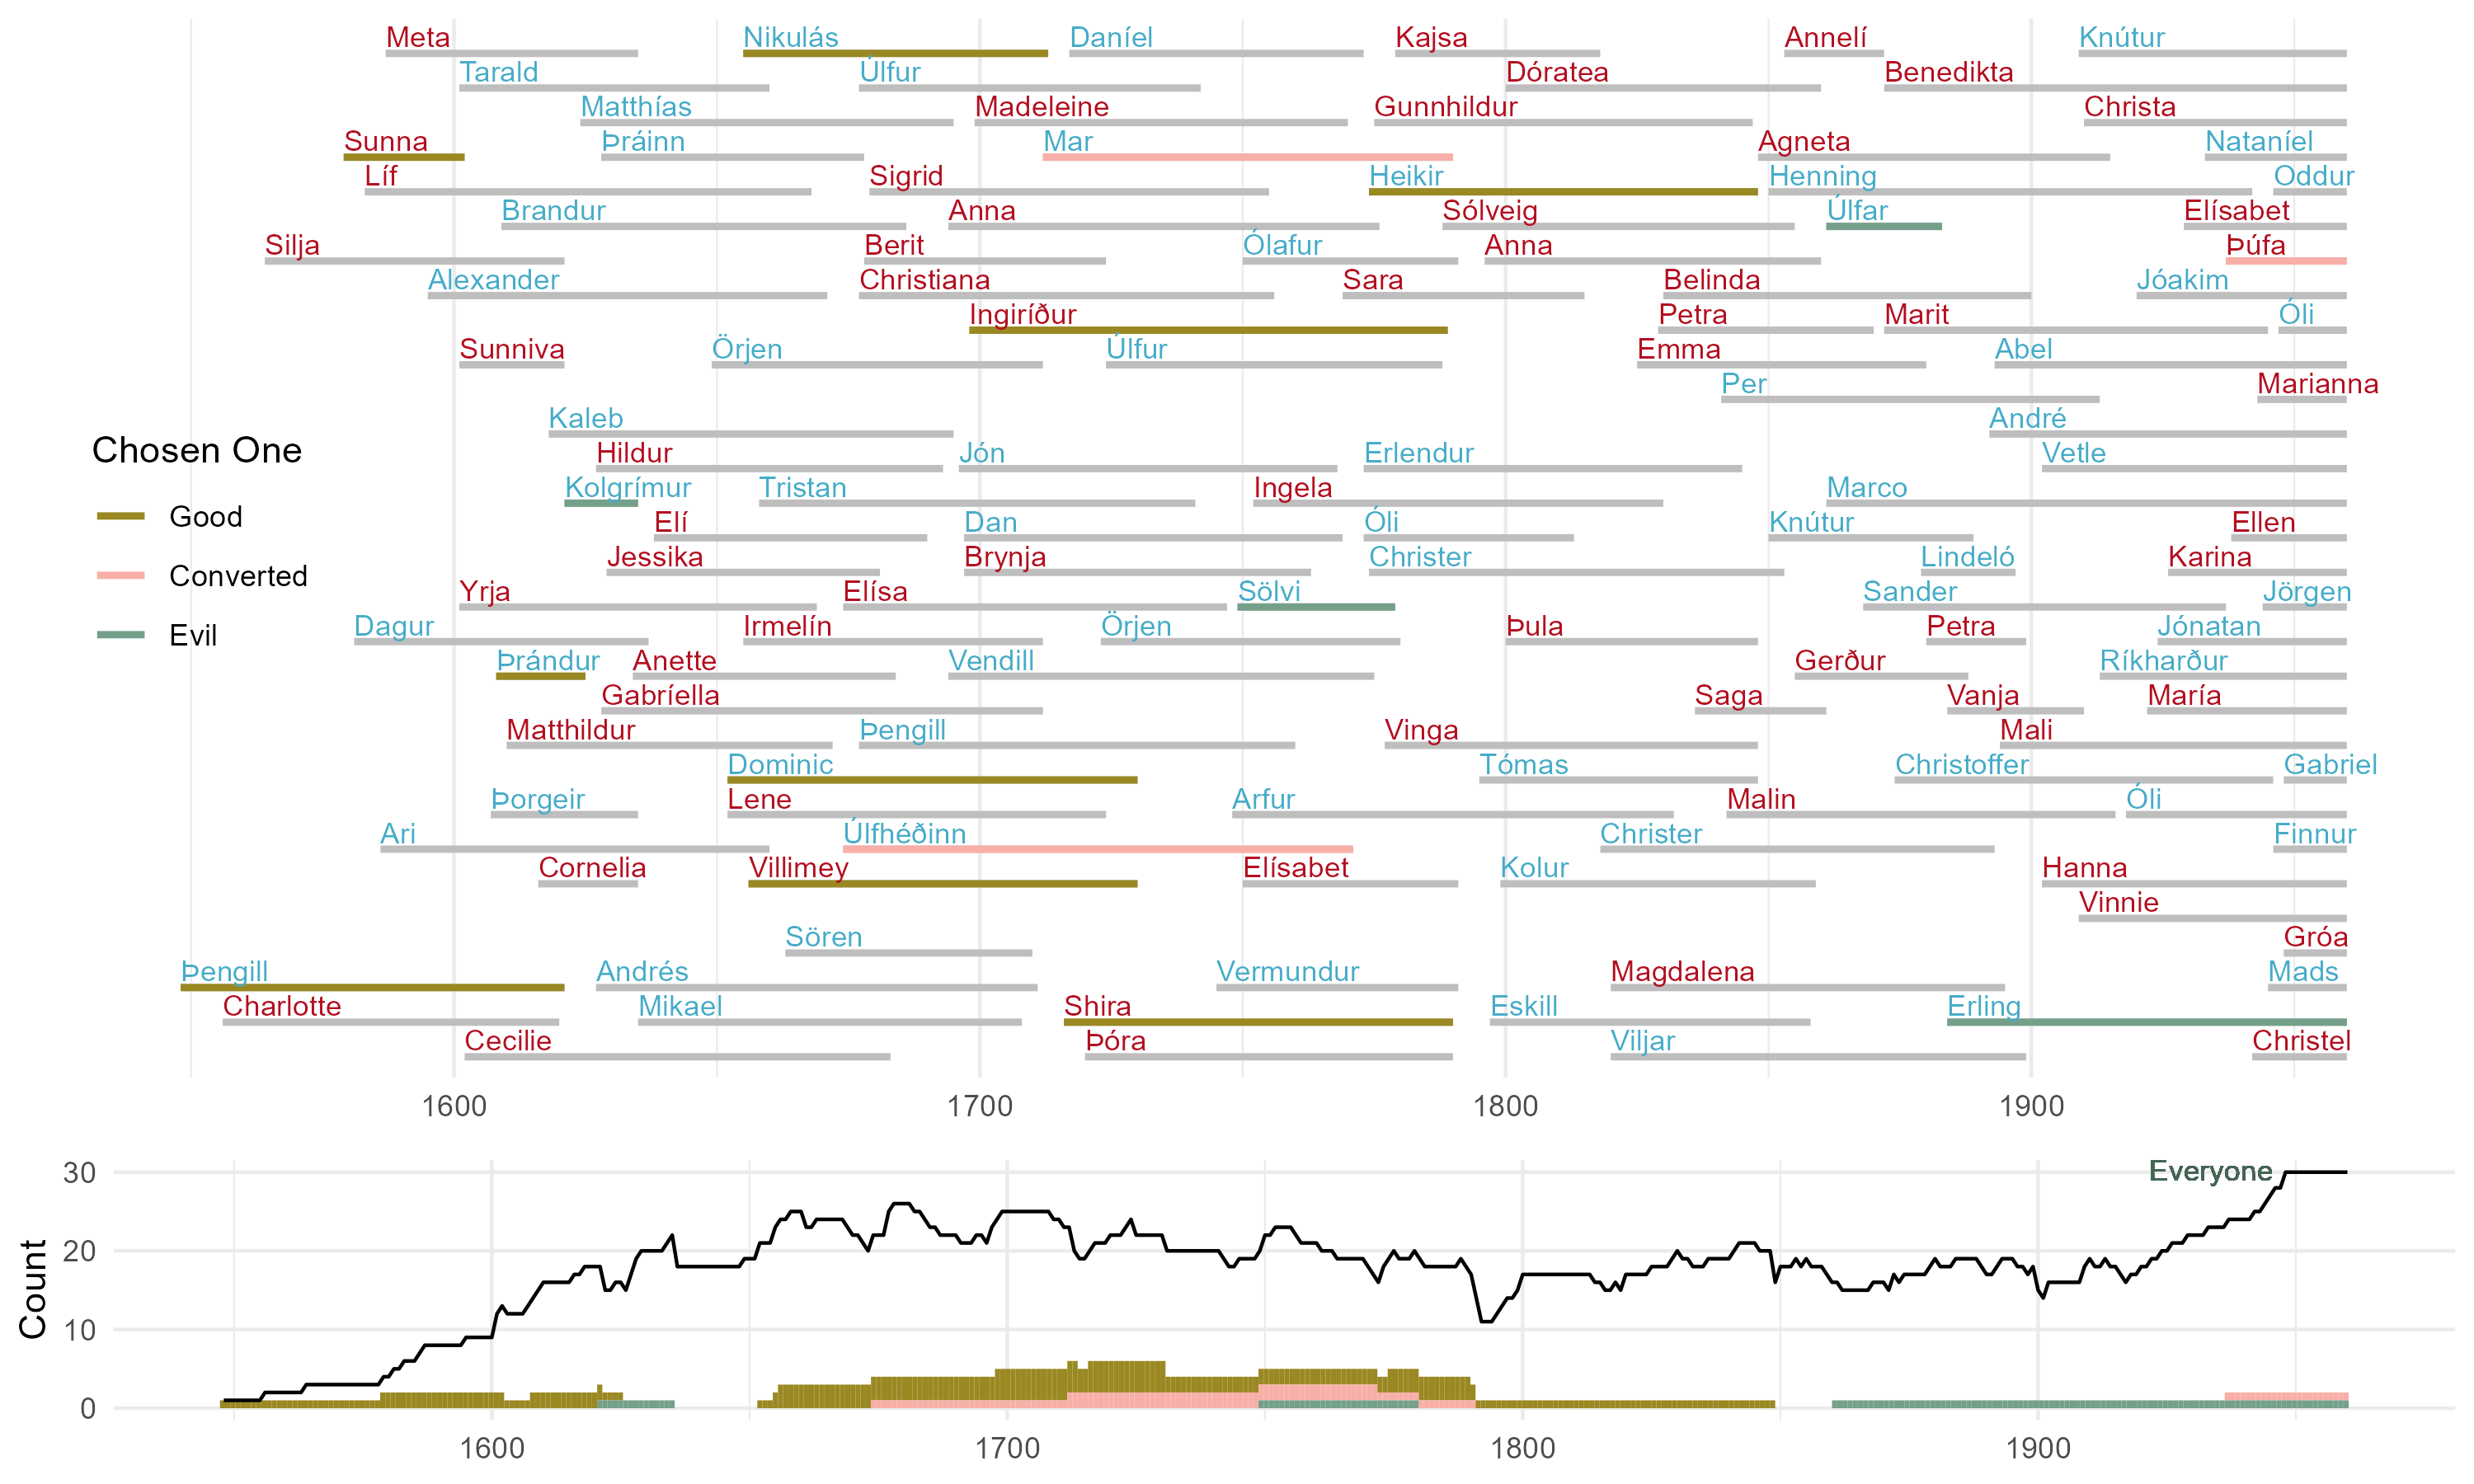
\includegraphics[width=\textwidth]{../R/figures/family_gantt}
\end{frame}

\begin{frame}{Lifespan of the Ice People}
\note{
\begin{itemize}
\item The data shows is a unique age \emph{bimodal distribution} diverging from the typical bell curve.
\item Many women, due to the curse, don't survive childbirth, leading to a life expectancy drop around the mid-20s.
\item Those women who overcome this hurdle often live up to 70 years, resulting in a second age peak.
\item Margit ensures symmetry: while women face childbirth peril, men, characterized by their recklessness, confront their own early-life dangers. Those men who navigate past these threats also enjoy an extended lifespan, reinforcing the bimodal pattern.
\item Looking at relationships:
 A third of characters are unrelated to the Ice People – or \emph{muggles}.
 Half are pure-bloods, having both parents from the Ice People.
 The rest, about 15\%, are half-bloods.
\end{itemize}
}

    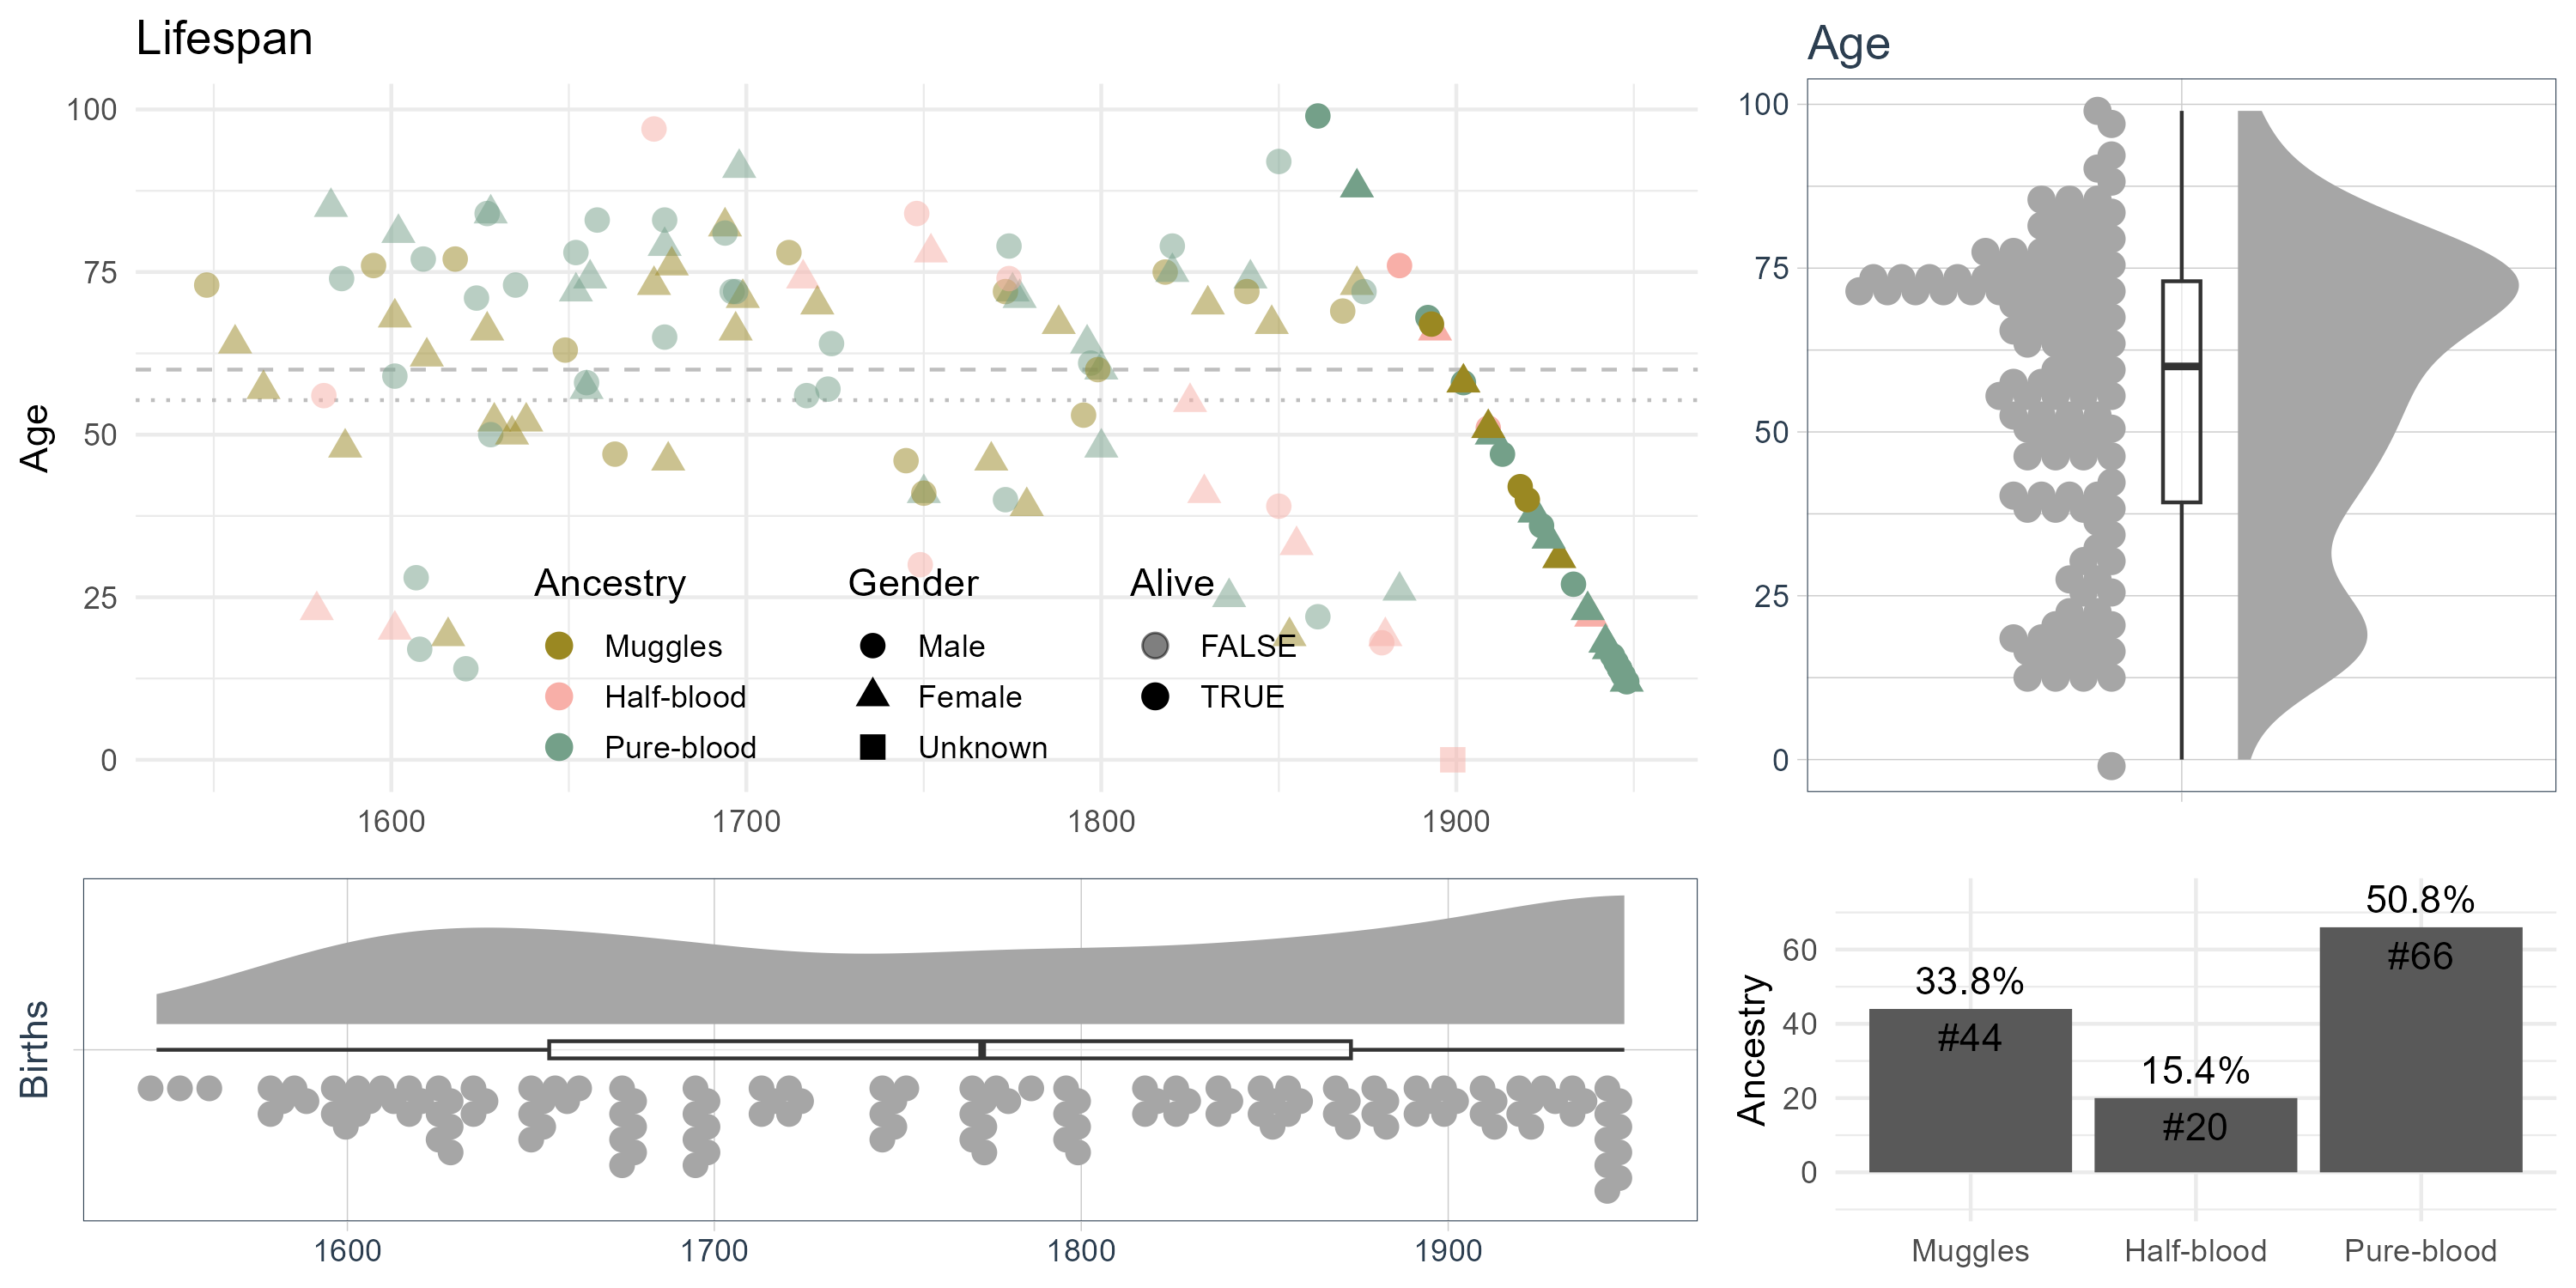
\includegraphics[width=\textwidth]{../R/figures/family_birth}
    \vspace{-18pt}
    \begin{itemize}
        \item Average woman lives 58.5 years (median 65, $n=50$)
        \item Average man lives 62.5 years (median 71, $n=49$)
        \item 1 centenarian, 4 people live to 90, 14 live to 80, 46 live to 70
    \end{itemize}
\end{frame}

\begin{frame}{Parental Age Trends \& Marital Age Gaps}
\note{
\begin{itemize}
\item Ice People women typically become mothers around 23.5 years, a choice influenced by prevalent dangers.
\item The curse dictates family size. One non-cursed child often stops family expansion, but a cursed birth may lead to larger families,
hoping the generation's \emph{curse quota} is filled.
\item Parental absence is a saga reality; a third of children grow up without a parent,
and it's not due to immaculate conceptions but the harsh reality of abandonment.
\item Yet, amidst these peculiarities, some aspects mirror our world. In 85\% of Ice People marriages, husbands are typically older by an average of three years — a trend not uncommon in our own society.

\end{itemize}
}    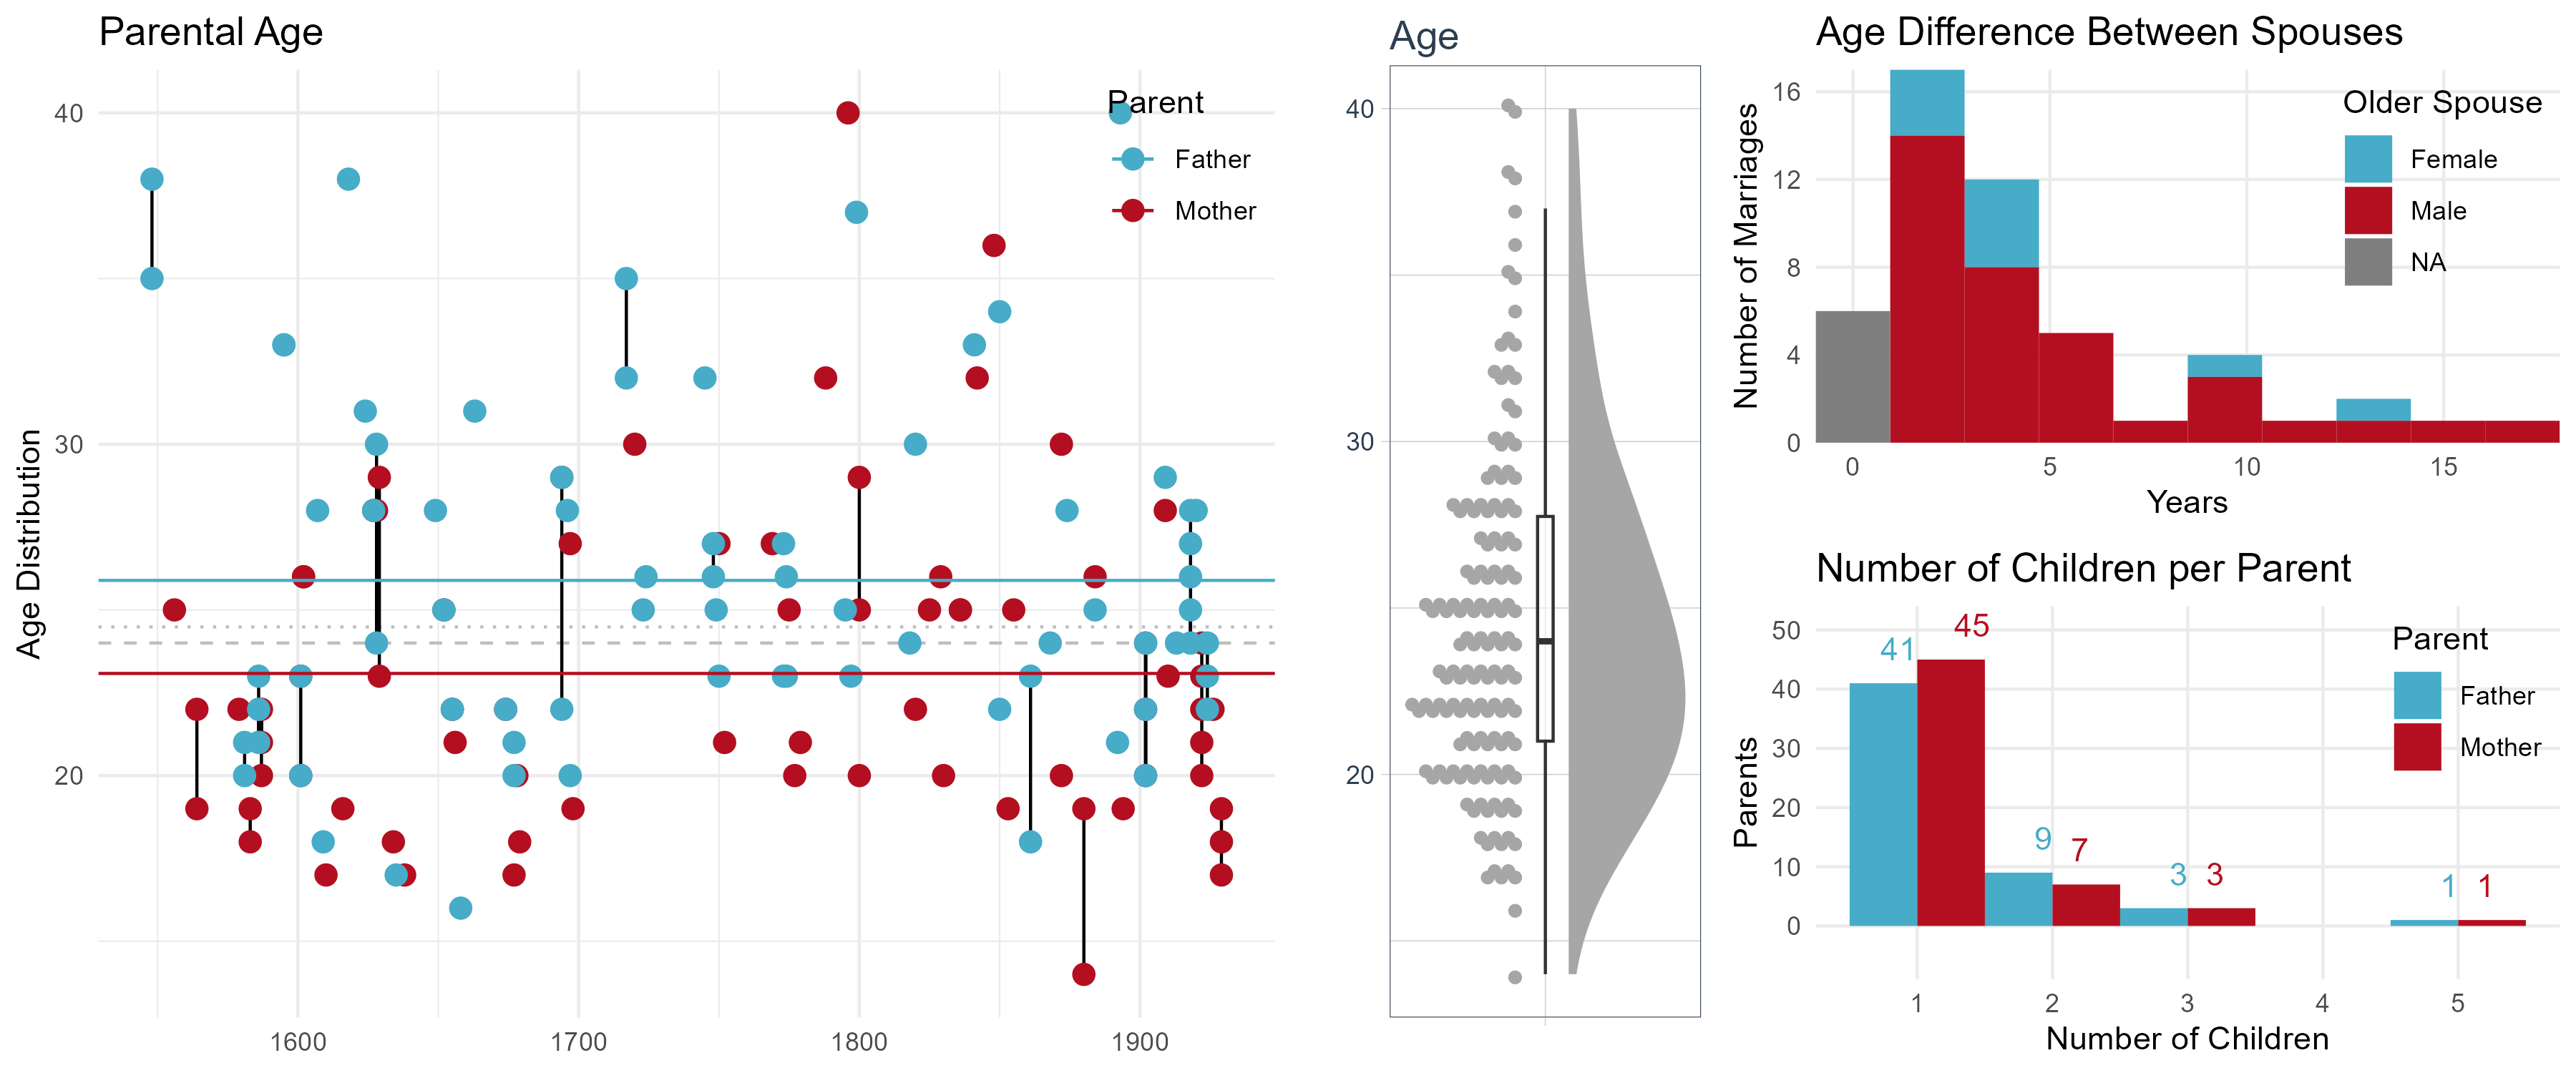
\includegraphics[width=\textwidth]{../R/figures/family_parent_age}
    \vspace{-18pt}
    \begin{itemize}
        \item 53 relationships described, 66 children born
        \item Average age of mother at childbirth is 23.5 years (fathers 26.0)
        \item 22 kids have either no father ($n=10$) or no mother ($n=12$)
        \item 85\% of marriages have an older husband, age difference generally 3 years (max 17 years)
    \end{itemize}
\end{frame}

\begin{frame}{Icelandic Naming Trends}
\note{\scriptsize
\begin{itemize}
\item In the 1980s, \emph{Ísfólkið} transcended literature, influencing Icelandic naming trends.
\item Names like \emph{Þula}, \emph{Yrja}, \emph{Heikir}, and \emph{Viljar} gained popularity post-publication, previously being unknown to Icelandic census.
\item There were significant surges: \emph{Sunna} increased 4-fold, \emph{Silja} doubled, and \emph{Saga} had a 5-fold jump.
\item Some name spikes, like \emph{Sölvi}, might be unrelated to the saga due to the character's malevolent nature.
\item However, names like \emph{Villimey} remained exclusive to the saga with no real-world adoptions.
\item Thanks to Yngvi Gautsson of \emph{Utopia Arctica} for the insightful data, helping clarify misconceptions from my earlier Reykjavík DataBeer Talk.
\end{itemize}
The saga's sway on Icelandic names emphasizes Margit's lasting cultural imprint.
}
    \centering
    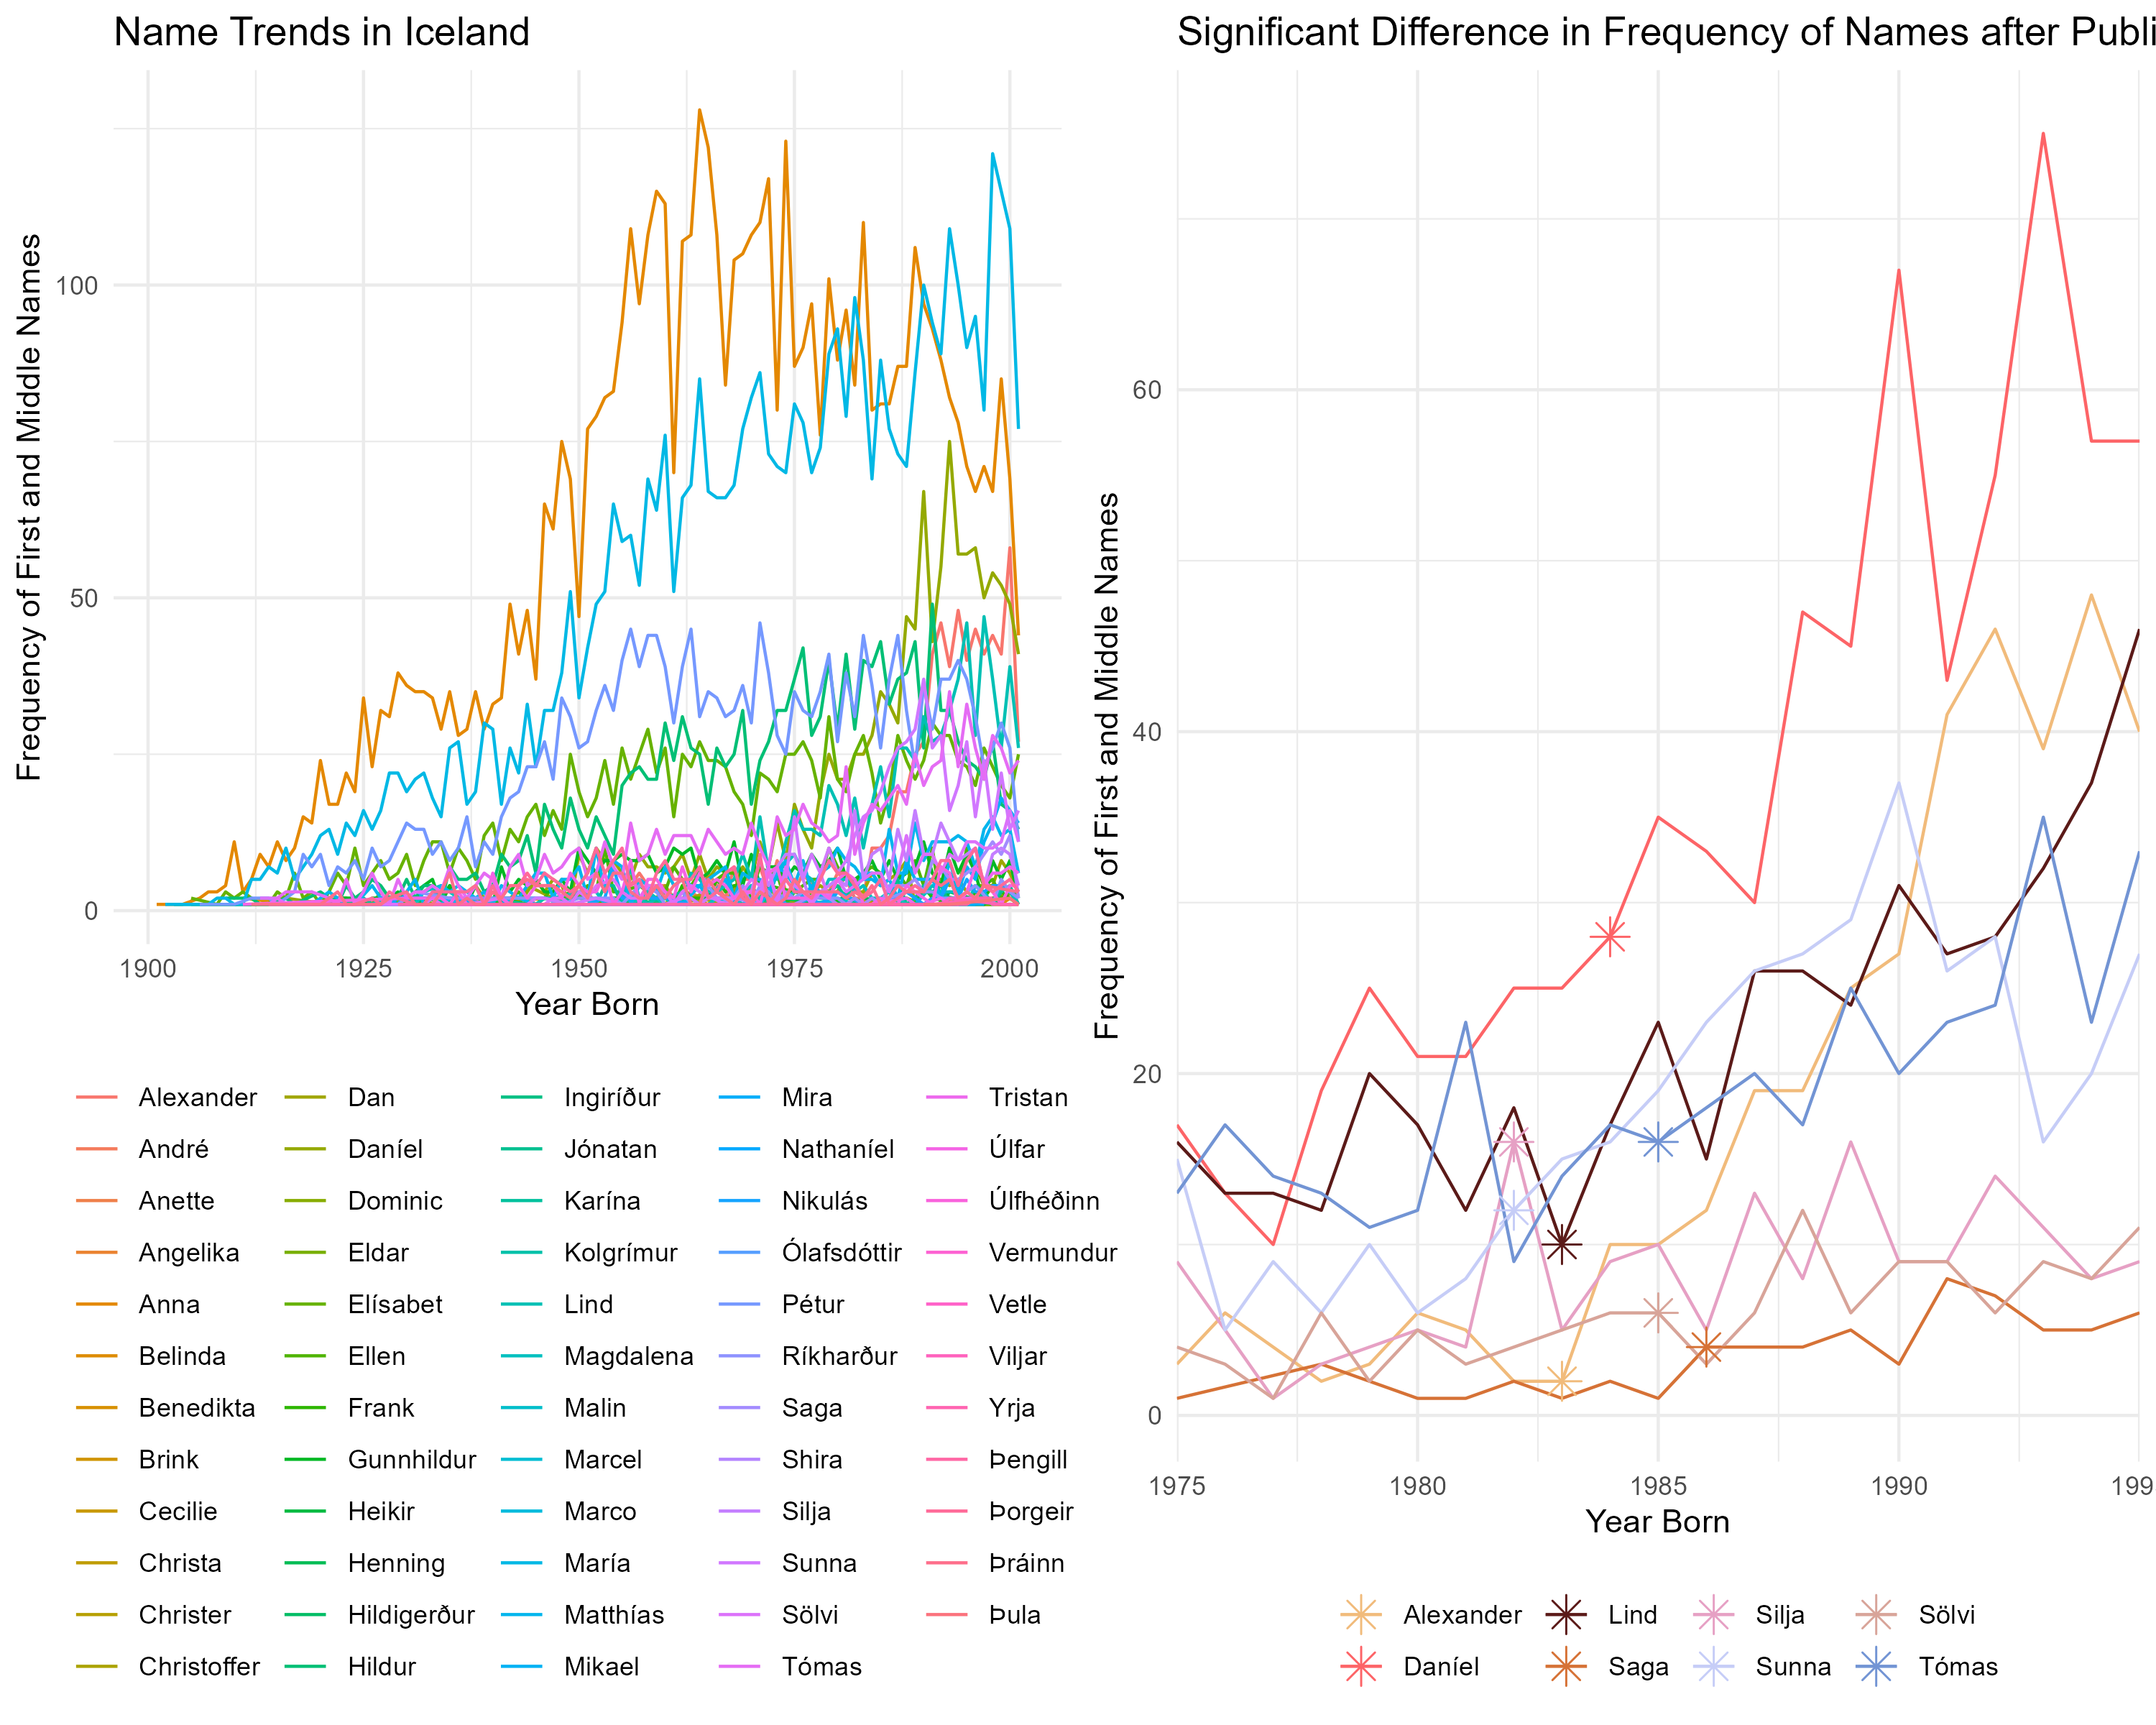
\includegraphics[width=\textwidth]{../R/figures/iceland_names.png}
    \vspace{-18pt}
    \begin{itemize}
        \item Protagonists' names \emph{Yrja}, \emph{Þula}, \emph{Heikir} and \emph{Viljar} first appear in the census
        a few years after Margit introduced them in her saga.
        \item Icelandic census data provided by Yngvi Gautsson of \emph{Utopia Arctica}
    \end{itemize}
\end{frame}


\section{Final Remarks}
\customframe[\note{\footnotesize
    \begin{itemize}
        \item While I'd have loved to be present, I'm currently in Italy, raising a glass to our \emph{ÍSKISUR} adventure alongside my incredible co-hosts.

        \item A huge thanks to Alvarpið and Storytel for granting us a platform to share our passion for \emph{Ísfólkið}.

        \item To our "\emph{only fan}" -- all four of you -- your spirited support has been invaluable.

        \item Heartfelt gratitude to the \emph{organizers} for offering me this stage today.

        \item Cheers to \emph{Reykjavík DataBeers} for igniting the data-driven exploration of \emph{Ísfólkið}.

        \item Immense appreciation for \emph{Margit}, whose work occupied four profound years of my life.

        \item To every \emph{listener}, thank you. I'm always open to discussions about data, \emph{Ísfólkið}, or cats!
        Feel free to touch base on Twitter, email, or explore the data available on GitHub.
        \end{itemize}
        \emph{Thank you!}
}
\begin{columns}[T]
    \begin{column}{0.6\textwidth}
        \tikz{
            \node[fill=white, fill opacity=0.5, text opacity=1, inner sep=5pt, align=left] {
                \begin{minipage}{\linewidth}
                    Feel free to contact me at \href{mailto:helgaingim@hi.is}{helgaingim@hi.is} \\
                    or \href{https://twitter.com/tungufoss}{@tungufoss} on Twitter. \\[12pt]
                    Get the source of this data analysis at: \\
                    \centering \url{github.com/tungufoss/iskisur-rek-data-beers} \\[6pt]
                    %\ccbysa % This requires the related package or command definition
                \end{minipage}
            };
        }
    \end{column}
    \begin{column} {0.3\textwidth}
        \href{https://www.youtube.com/watch?v=DK7CVqbtW0A}{
            
\includegraphics[width=\textwidth]{../rek-data-beers/figures/dalle-keyboardcat}
        }
    \end{column}
\end{columns}
]{../rek-data-beers/figures/dalle-book-1}{Thank You}

\end{document}
